\documentclass[aps,pra, twocolumn]{revtex4}
\usepackage{amssymb,amsthm,amsmath,enumerate,url, graphicx, float, csvsimple, todonotes, enumitem}

\def\FCW{1.0\columnwidth}

\newcommand{\multi}[1]{\vec{#1}}
\newcommand{\bs}[1]{\boldsymbol{#1}}
\newcommand{\pr}{\mathrm{Pr}}
\newcommand{\pdiff}[2]{\frac{\partial #1}{\partial #2}}
\renewcommand{\d}{\mathrm{d}}
\newcommand{\M}{\mathcal{M}}
\newcommand{\R}{\mathcal{R}}
\newcommand{\Tr}{\mathrm{Tr}}
\newcommand{\Lik}{\mathcal{L}}
\renewcommand{\P}{\mathcal{P}}
\newcommand{\stup}{\uparrow}
\newcommand{\stdown}{\downarrow}
\newcommand{\stleft}{\leftarrow}
\newcommand{\stright}{\rightarrow}
\newcommand{\styplus}{\nearrow}
\newcommand{\styminus}{\swarrow}
\newcommand{\reals}{\mathbb{R}}
\newcommand{\cH}{\mathcal{H}}
\newcommand{\cL}{\mathcal{L}}
\newcommand{\ket}[1]{\ensuremath{\left|#1\right\rangle}}
\newcommand{\bra}[1]{\ensuremath{\left\langle\scriptstyle#1\right|}}
\newcommand{\braket}[2]{\ensuremath{\left\langle\scriptstyle#1|#2\right\rangle}}
\newcommand{\ketbra}[2]{\ket{#1}\!\!\bra{#2}}
\newcommand{\expect}[1]{\ensuremath{\left\langle#1\right\rangle}}
\newcommand{\braopket}[3]{\ensuremath{\bra{#1}#2\ket{#3}}}
\newcommand{\proj}[1]{\ketbra{#1}{#1}}
\newcommand{\union}{\cup}
\def\Id{1\!\mathrm{l}}
\newcommand{\Fi}{\mathcal{I}}

\newcommand{\bvec}[1]{\boldsymbol{#1}}
 

\newcommand{\rhohat}{\hat{\rho}}
\newcommand{\rhoBME}{\rhohat_{\scriptscriptstyle\mathrm{BME}}}
\newcommand{\rhoMLE}{\rhohat_{\scriptscriptstyle\mathrm{MLE}}}
\newcommand{\rhotomo}{\rhohat_{\scriptscriptstyle\mathrm{tomo}}}
\newcommand{\rhotrue}{\rho_{\scriptscriptstyle\mathrm{true}}}
\newcommand{\phat}{\hat{p}}

\newcommand{\diff}{\mathrm{d}\!}
\newcommand{\diffk}[1]{\mathrm{d}_{#1}\!}

\begin{document}
\author{Travis L Scholten}
\author{Robin Blume-Kohout}
\affiliation{Center for Computing Research (CCR), Sandia National Labs \emph{and} University of New Mexico}

\title{Behavior of the Maximum Likelihood in Quantum State Tomography}

\begin{abstract}
Quantum state tomography on a $d$-dimensional system demands resources that grow rapidly with $d$. Model selection can be used to tailor the number of fit parameters to the data, but quantum tomography violates some common assumptions that underly canonical model selection techniques based on ratios of maximum likelihoods (loglikelihood ratio statistics), due to the nature of the state space boundaries. Here, we study the behavior of the maximum likelihood  in different Hilbert space dimensions, and derive an expression for a complexity penalty -- the expected value of the loglikelihood ratio statistic (roughly, the logarithm of the maximum likelihood) -- that can be used to make an appropriate choice for $d$.
\end{abstract}
\date{\today}

\maketitle

In quantum information science, an experimentalist may wish to determine the quantum state $\rho_{0}$ that is produced by a specific initialization procedure.  This can be done using quantum state tomography \cite{Paris2004}:  many copies of $\rho_{0}$ are produced; they are measured in diverse ways; and finally the outcomes of those measurements (data) are collated and analyzed to produce an estimate $\rhohat$.  This is a straightforward statistical inference process \cite{Reid2015, Wasserman2004}, where the data are used to fit the parameters of a statistical model -- provided that we know what statistical model to use.  But this is not always the case.  In state tomography, the parameter is $\rho$, and the model is the set of all possible density matrices on a Hilbert space $\cH$ (equipped with the Born rule). It is not always \emph{a priori} obvious what $\cH$ or its dimension is; examples include optical modes \cite{Altepeter2005, Bertrand1987, Lvovsky2009, Breitenbach1997, Leonhardt1995} and leakage levels in AMO and superconducting \cite{Motzoi2009, Fazio1999} qubits.  Choosing an appropriate Hilbert space on the fly is \emph{model selection}, and while model selection is well-studied in classical statistics \cite{Burnham2004}, applying it to quantum tomography leads to some surprising twists.  These problems stem from the positivity constraint ($\rhohat\geq0$). The techniques we use to resolve them are relevant not just to model selection, but to quantum tomography on low-rank states.

Many methods for selecting between multiple models involve fitting each model's parameters using \emph{maximum likelihood estimation} (MLE) \cite{Hradil1997, JamesPRA2001, Blume-Kohout2010}, which reports the parameter values that maximize the likelihood (the probability of the observed data). Classical estimation problems usually satisfy \emph{local asymptotic normality} \cite{LeCam1970, LeCam1956}, meaning that: (1) as $N_{\mathrm{samples}}\rightarrow \infty$,  $\rhoMLE$ is normally distributed around the true state $\rho_{0}$ with covariance matrix $\Fi^{-1}$, and (2) the likelihood function in a neighborhood of $\rhoMLE$ is locally Gaussian with Hessian $\Fi$, where $\Fi$ is the \emph{Fisher information}.

\begin{figure}[h]
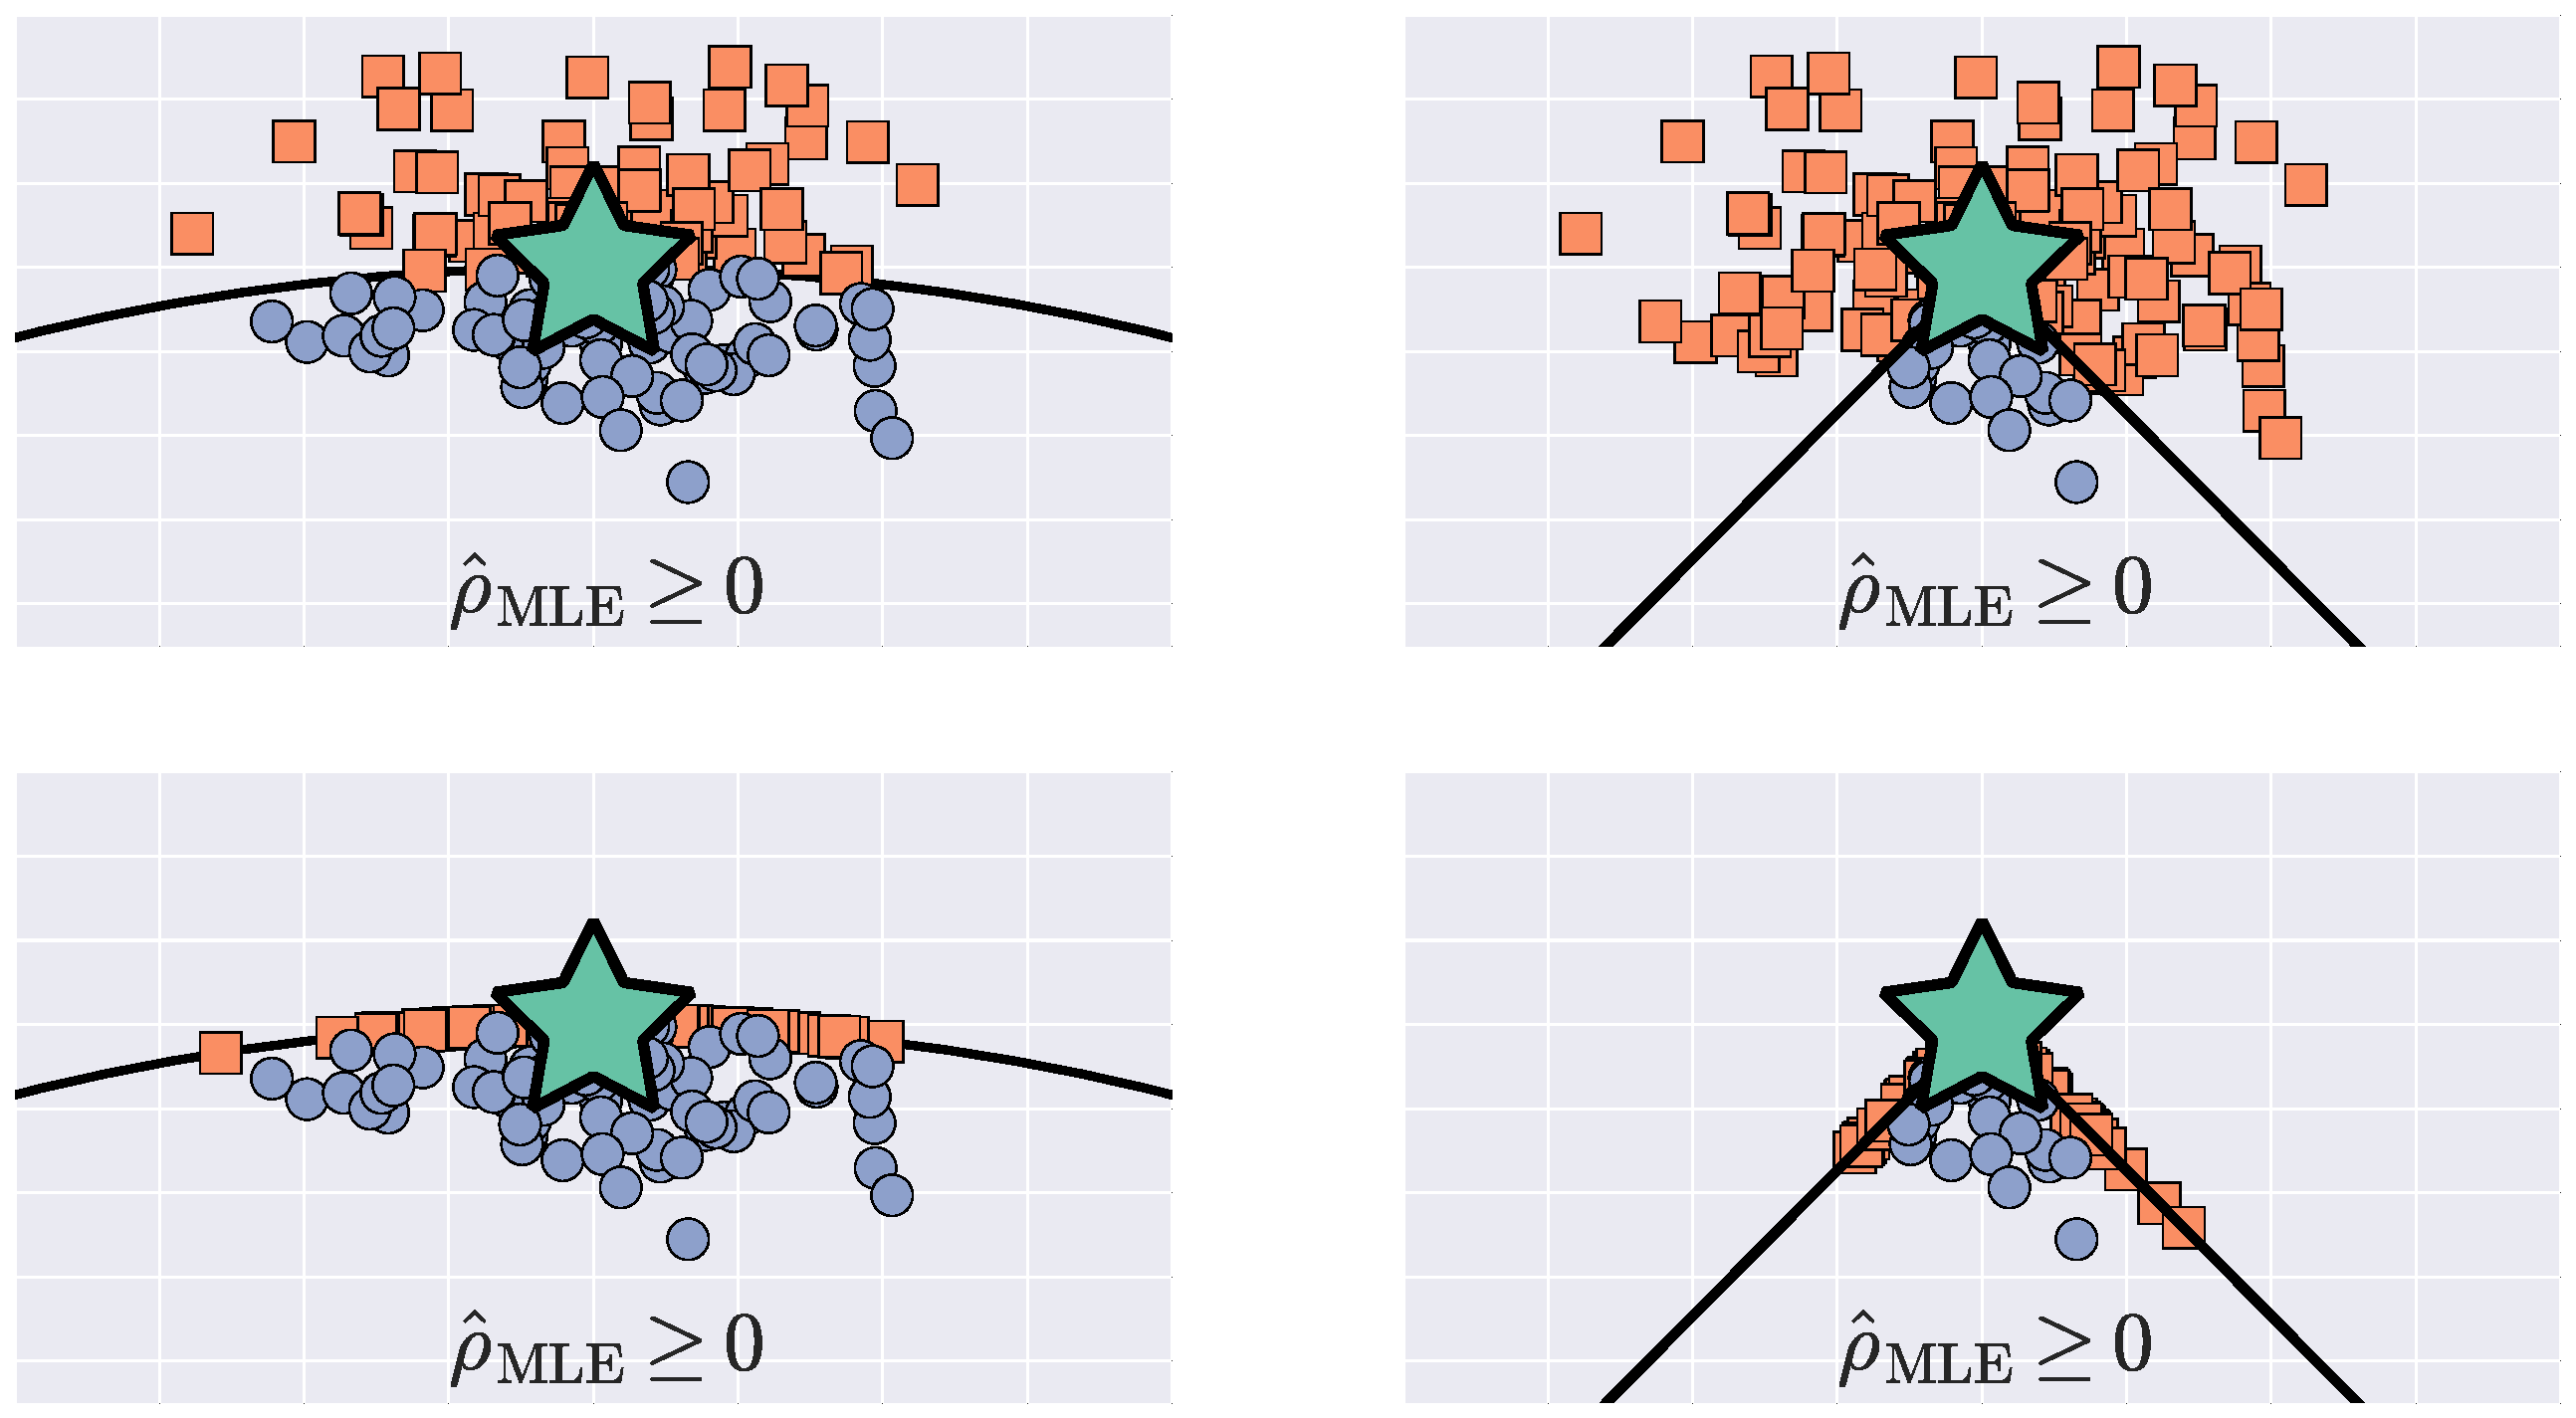
\includegraphics[width=\columnwidth]{Images/Figure_1.pdf}
 \caption{Impact of the boundary on maximum likelihood tomography. \textbf{Top}: Two views through the qutrit state space. Without the positivity constraint, some estimates (orange squares) are not positive semidefinite, and do not represent valid estimates of a quantum state. The distribution of $\rhoMLE$ (blue circles) is generally non-normal, and depends on the true state $\rho_{0}$ (star).
\textbf{Bottom}:  Comparison of the classical theory (Wilks Theorem) prediction for the loglikelihood ratio $\expect{\lambda}$ to numerical data for true states of rank $r=1\ldots 10$.  The Wilks Theorem fails badly for low-rank states; our main result (Equation \ref{eq:ourLLRS}) fixes this problem (see Figure \ref{fig:modelcomp-iso}).}
\label{fig:boundaries}
\end{figure}

In state tomography, these conditions are violated by the constraint $\rhoMLE \geq 0$. This constraint distorts the distribution of estimates, even in the asymptotic limit, precisely when $\rho_{0}$ is rank-deficient within $\cH$. (That is, when $\rho_{0}$ is on the boundary of $\cH$. See Figure \ref{fig:boundaries}.) While the behavior of MLEs is well-studied classically, its behavior near boundaries is not.  How boundaries affect $\rhoMLE$ -- and its derived properties -- is of broad interest in state and process tomography  \cite{Candes2006, Flammia2012a}, and is also critical for model selection \cite{Schwarz2013a, Guta2012a, VanEnk2013a, Yin2011, Moroder2013}.



We will focus on the special and simple case where $\Fi$ at $\rho_{0}$ is  proportional to the Hilbert-Schmidt metric, so the likelihood function (and the distribution of the \emph{unconstrained} estimates $\rhohat$) is given by 
\begin{equation}
\label{eq:likelihood}
\cL(\rho) = \mathrm{Pr}(\rhohat | \rho) \propto e^{-||\rho - \rhohat||^{2}_{2}/2\epsilon^{2}}
\end{equation}
for some $\epsilon$ that scales as $1 / \sqrt{N_{\mathrm{samples}}}$.  In practice, $\Fi$  depends  on $\rho_{0}$ and the particular tomographic measurement performed, but the interaction of an arbitrary Fisher information with the boundary is complex and intractable. The isotropic assumption greatly simplifies our study of the problem, and permits the derivation of analytic results which capture realistic tomographic scenarios surprisingly well \cite{Smolin2012}.

In this case, $\rhohat$ is often not positive semidefinite (see Figure \ref{fig:boundaries}). For each such $\rhohat$, the actual $\rhoMLE$ is the solution to the following optimization problem:
\begin{equation}
\label{eq:mleopt}
\rhoMLE = \underset{\substack{\rho \in \mathcal{B}(\cH)  \\ \mathrm{Tr}(\rho)=1, \rho \geq 0}}{\mathrm{argmin}}~\mathrm{Tr}[(\rhohat - \rho)^{2}],
\end{equation}
and the distribution of $\rhoMLE$ is not generally normal. We do not attempt to derive $\mathrm{Pr}(\rhoMLE)$ explicitly. Instead, we demonstrate a method for computing the behavior of useful statistics which depend on $\rhoMLE$, such as the expected value of the loglikelihood ratio statistic $\langle \lambda \rangle$, a key quantity in model selection.

%----------MODEL SELECTION-------------%
Model selection becomes relevant when several candidate models could be fit to the data.  A model's ``size'' is the number of free parameters in it, and as a general rule, the best model is the smallest one that fits the data well.  Many model selection techniques use a statistic to quantify goodness of fit; a commonly used statistic is the \emph{loglikelihood ratio} \cite{Blume-Kohout2010, Moroder2013, Neyman1933},
\begin{equation}
\lambda(\M_{1}, \M_{2}) = -2 \log \left(\frac{\underset{\rho \in \M_{1}}{\max}~\cL(\rho)}{\underset{\rho \in 
\M_{2}}{\max}~\cL(\rho)}\right).
\end{equation}
Intuitively, the model with the higher likelihood is more plausible -- except that models with 
more adjustable parameters will almost always fit the data better!  This is very clear in the case
of \emph{nested} models ($\M_{1}$ is a submanifold of $\M_{2}$) \footnote{If $\M_{1}\subset \M_{2}$, then the maximum likelihood of $\M_{2}$ is at least as high as that of $\M_{1}$.}. If two models are equally valid -- i.e. they both contain the true state $\rho_0$ -- the larger one will usually fit the data better because its extra parameters allow it to fit more of the noise in the data.  For the same reason, the larger model's fit will be less accurate.  This makes it imperative to correct for overfitting, by handicapping larger models.

For this reason, any model selection method that relies (explicitly or implicitly) on a statistic to quantify ``how well model $\M$ fits the data'' also relies on a \emph{null theory} to predict how that statistic will behave \emph{if} $\rho_{0} \in \M$.  A model selection criterion based on an invalid null theory (or a criterion used in a context where its null theory does not apply) will tend to choose the wrong model. When local asymptotic normality holds, the null theory for $\lambda$ is given by the \emph{Wilks Theorem} \cite{Wilks1938}: if $\rho_{0}\in \M_{1}\subset \M_{2}$, where $\M_{1}$ has $k$ free parameters and $\M_{2}$ has $K+k$ free parameters, then $ \lambda$ is a $\chi^{2}_{K}$ random variable, so that $\expect{\lambda} = K$.

Consider using model selection to evaluate a particular $d$-dimensional Hilbert space $\cH_{d}$, by comparing $\cH_{d}$ to $\cH_{d+1}$ using $\lambda$. We define the model $\mathcal{M}_{d}$ (for any $d$) as
\begin{equation}
\mathcal{M}_{d} = \{\rho~|~\rho \in \mathcal{B}(\mathcal{H}_{d}),~\mathrm{Tr}(\rho) =1,~\rho \geq 0\},
\end{equation}
where $\mathcal{B}(\cH)$ is the space of bounded operators on $\cH$.
Now, before we can use the observed value of $\lambda$ to decide whether $\mathcal{H}_{d+1}$ is significantly better, we need a null theory for its behavior when it \emph{isn't} better (i.e., when $\rho_{0}$ is in both $\mathcal{M}_d$ and $ \mathcal{M}_{d+1}$). In what follows, it's useful to reduce the problem of computing $\lambda(\M_{d}, \M_{d+1})$ to that of computing $\lambda(\rho_{0}, \M_{d})$ and $\lambda(\rho_{0}, \M_{d+1})$ using the identity
\begin{equation}
\lambda(\mathcal{M}_{d}, \mathcal{M}_{d + 1}) = \lambda(\rho_{0}, \mathcal{M}_{d+1}) - \lambda(\rho_{0}, \mathcal{M}_{d}),
\end{equation}
where
\begin{equation}
\label{eq:llrs}
\lambda(\rho_{0}, \mathcal{M}_{d}) = -2 \log \left(\frac{\mathcal{L}(\rho_{0})}{\underset{\rho \in \mathcal{M}_{d}}{\max}
\mathcal{L}(\rho)}\right).
\end{equation}
When $\rho_{0}$ is full-rank, the Wilks Theorem applies, and  $\lambda \sim \chi^{2}_{d^{2}-1}$ \footnote{Because $\rho_{0}$ is \emph{fixed}, the number of free parameters is 0.}. However, the behavior of $\lambda$ depends crucially on the \emph{rank} of $\rho_{0}$. If $\rho_{0}$ is rank-deficient, then the boundary looms, local asymptotic normality does not hold, and the Wilks Theorem does not apply! Even if $\rho_{0}$ is full-rank in $\M_{d}$, it will be rank-deficient in $\M_{d+1}$. Thus, to do model selection for Hilbert space dimension in state tomography, we must understand the null behavior of $\lambda(\rho_{0}, \M_{d})$ -- i.e., derive a replacement Wilks Theorem -- for rank-deficient $\rho_{0}$.  Some of the more technical details of this derivation are deferred to Appendix \ref{app:technical} in the Supplementary Material.

%----------DERIVING A WILKS REPLACEMENT--------------%
In our derivation, we assume that $\rho_{0}, \rhoMLE \in \M_{d}$, that $r \equiv \mathrm{Rank}(\rho_{0}) < d$, and that the Fisher information at $\rho_0$ is $\Fi  = \epsilon^{2} \Id$.  The loglikelihood ratio that we're trying to predict is equal to $\lambda(\rho_0, \rhoMLE) = \epsilon^{-2}\Tr{[(\rhoMLE - \rho_{0})^2]}$, where $\rhoMLE$ is the MLE over $\M_{d}$.  The \emph{unconstrained} estimates are distributed as $\mathrm{Pr}(\rhohat) = \mathcal{N}(\rho_0,\epsilon^2\Id)$. 

We need a procedure to compute $\rhoMLE$ given $\rhohat$ -- i.e., to solve the optimization problem in Eq. \eqref{eq:mleopt}.  Fortunately, for the special case of isotropic Fisher information, this problem was solved in Ref. \cite{Smolin2012}:
\begin{enumerate}[noitemsep]
\item Subtract $q\Id$ from the unconstrained $\hat\rho$, for a particular real scalar $q$,
\item ``Truncate'' $\hat\rho-q\Id$, by replacing each of its negative eigenvalues with zero.
\end{enumerate}
Here, $q$ is defined implicitly such that $\Tr\left[ \mathrm{Trunc}(\hat\rho-q\Id)\right] = 1$.

Although this was intended as a (very fast) numerical algorithm, we will abuse it (by a series of approximations) to derive a closed-form expression for the average $\expect{\lambda}$.  We begin by observing that $\lambda(\rho_{0}, \rhoMLE)$ can be written as a sum over matrix elements,
\begin{align}
\label{eq:llrserrors}
\nonumber \lambda &=\epsilon^{-2}\mathrm{Tr}[(\rhoMLE - \rho_{0})^{2}] = \epsilon^{-2}\sum_{jk}|(\rhoMLE- \rho_{0} )_{jk}|^{2}\\
&= \sum_{jk}\lambda_{jk}~~~~\text{where}~~~~\lambda_{jk} = \epsilon^{-2}|(\rhoMLE - \rho_{0} )_{jk} |^{2},
\end{align}
and therefore $\langle \lambda \rangle = \sum_{jk}\langle\lambda_{jk}\rangle$.  Each term $\langle \lambda_{jk}\rangle$ quantifies the average mean-squared error of a single matrix element of MLE, and while the Wilks Theorem predicts $\expect{\lambda_{jk}}=1$ for all $j,k$, numerical simulations (see Fig. \ref{fig:L}) show that this only holds true for \emph{some} matrix elements.  A few contribute more than 1 unit (on average) while many others contribute much less, meaning that the Wilks Theorem predicts too high a value for the total $\expect{\lambda}$.  Thus motivated, we divide the parameters of $\rhohat$ into two parts (see Fig. \ref{fig:L}),
\begin{enumerate}[noitemsep]
\item The ``kite'' comprises all diagonal elements \emph{and} all elements on the kernel (null space) of $\rho_0$,
\item The ``L'' comprises all off-diagonal elements on the support of $\rho_0$ \emph{and} between the support and the kernel,
\end{enumerate}
and observe that $\langle\lambda\rangle = \expect{\lambda}_{\mathrm{L}} + \expect{\lambda}_{\mathrm{kite}}$.  The rationale for this division is simple:  small fluctuations on the ``L'' do not change the zero eigenvalues of $\hat\rho$ to 1st order, whereas those on the ``kite'' do.    

\begin{figure}[h]
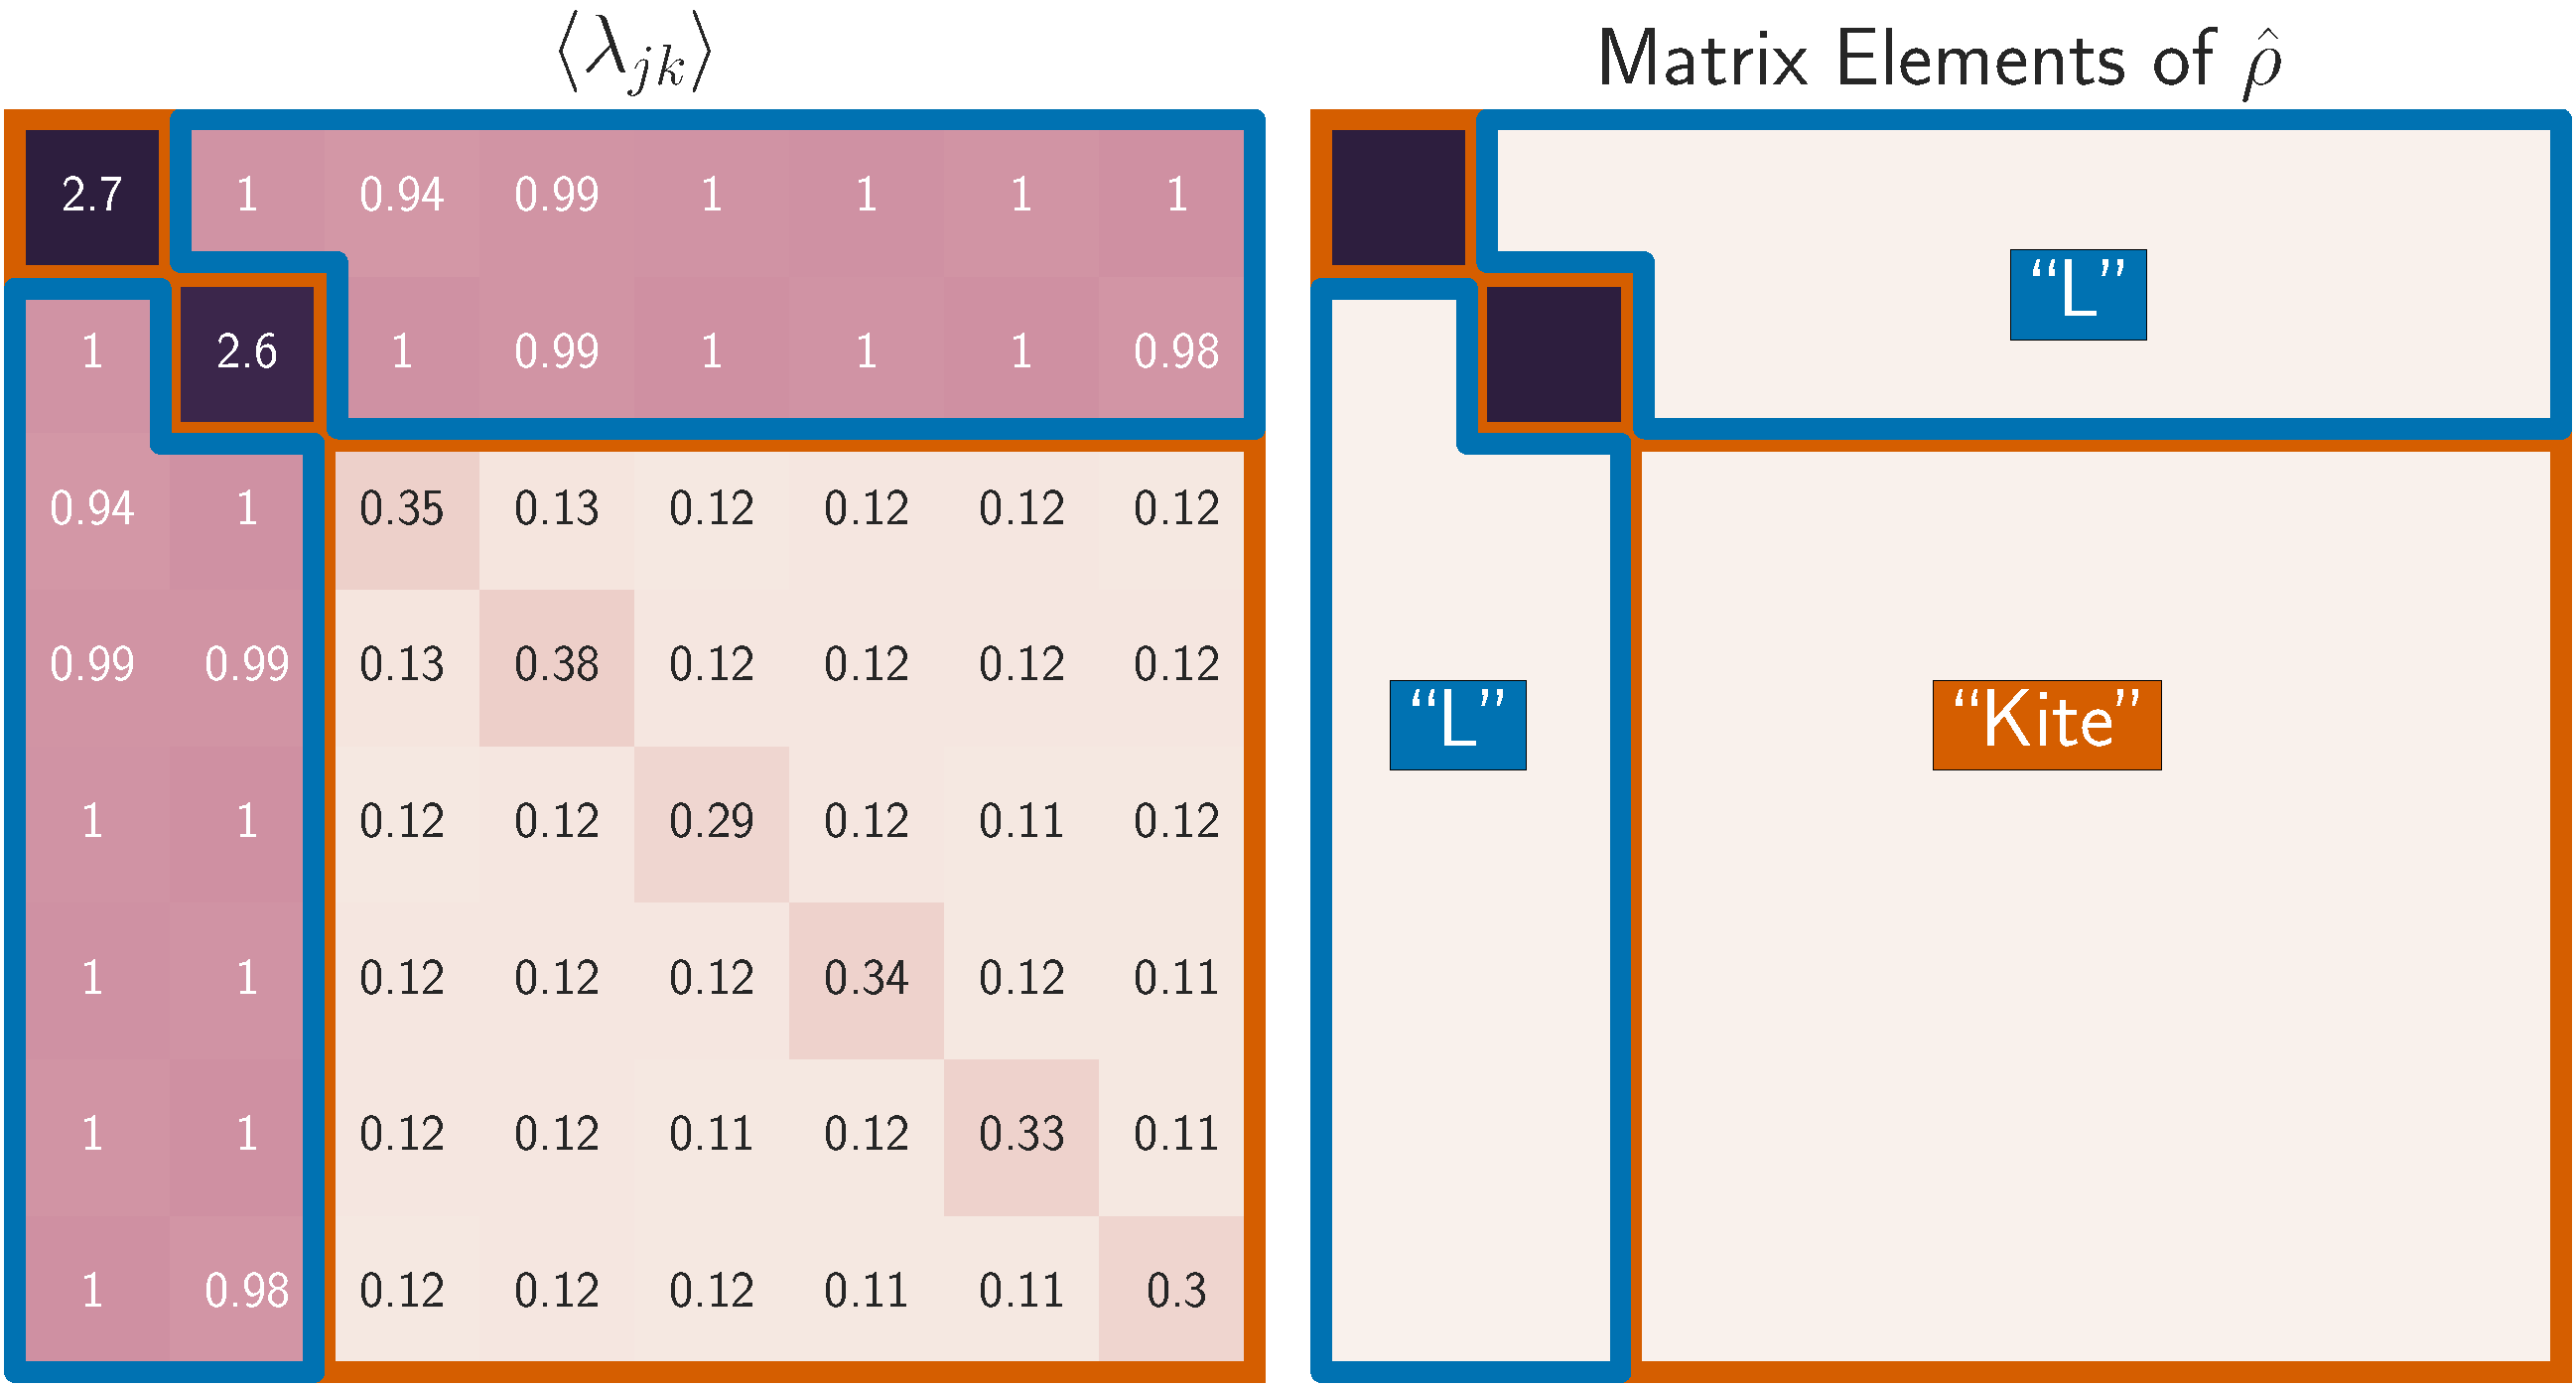
\includegraphics[width=\columnwidth]{Images/Figure_2.pdf}
 \caption{When a rank-2 state is reconstructed in $d=8$ dimensions, the total loglikelihood ratio $\lambda(\rho_0,\mathcal{M}_8)$ is the sum of contributions $\lambda_{jk}$ from errors in each matrix element $(\rhoMLE)_{jk}$.  \textbf{Left}:  Numerics show a clear division; some matrix elements contribute $\expect{\lambda_{jk}}\sim1$ as predicted by the Wilks Theorem, while others contribute either more or less. \textbf{Right}:  The numerical results motivate dividing the elements of $\rhohat$ into two parts: the ``kite'' and the ``L''.}
\label{fig:L}
\end{figure}

The error of the unconstrained estimate is $\delta = \hat\rho- \rho_{0}$, a normally-distributed \emph{traceless} matrix.  To simplify the analysis, we explicitly drop the $\Tr(\rho)=1$ constraint and let $\delta$ be $\mathcal{N}(0,\epsilon^2\Id)$ distributed over the $d^2$-dimensional space of Hermitian matrices (a good approximation when $d\gg2$), which makes $\delta$ proportional to an element of the Gaussian Unitary Ensemble (GUE) \cite{Fyodorov2005}.  

Now, to first order in $\epsilon$, elements of $\delta$ in the ``L'' do not affect positivity, so they are unconstrained by the boundary, and behave exactly as expected from classical theory. This is because the $\delta_{jk}$ in the ``L'' may be seen as errors which arise due to small unitary perturbations of the true state $\rho_{0}$. Writing $\rhohat = U^{\dagger}\rho_{0}U$, where $U=e^{i\epsilon H}$, we have
\[\rhohat \approx \rho_{0} + i\epsilon [\rho_{0},H]+\mathcal{O}(\epsilon^{2}).\]
Then, $\delta \approx i\epsilon [\rho_{0},H]$.
If $j = k$, then $\delta_{jj} = 0$. Thus, small unitaries cannot create errors in the diagonal matrix elements, at $\mathcal{O}(\epsilon)$. If $j \neq k$, then $\delta_{jk} \neq 0$, in general. So small unitaries \emph{can} introduce errors on off-diagonal elements.

However, if either $\ket{j}$ or $\ket{k}$ (or both) lie within the \emph{kernel} of $\rho_{0}$ (i.e., $\rho_{0}\ket{k}$ or $\rho_{0}\ket{j}$ is equal to 0), then the corresponding $\delta_{jk}$ are zero. The only off-diagonal elements where small unitaries can introduce errors are those which are coherent between the kernel of $\rho_{0}$ and its support. These off-diagonal elements are precisely the ``L", and are  the set $\{\delta_{jk}~|~\langle j | \rho_{0}|j\rangle \neq 0, j\neq k, ~ 0 \leq j,k \leq d - 1\}$. Each $\delta_{jk}$ in the ``L'' has Gaussian fluctuations and so for those elements, $\langle \lambda_{jk} \rangle = 1$. As there are $2rd - r(r+1)$ of them in the ``L", $\expect{\lambda}_{\mathrm{L}} = 2rd - r(r+1)$.

Computing $\expect{\lambda}_{\mathrm{kite}}$ is a bit harder, because the boundary \emph{does} constrain elements in the ``kite''.  Here, we turn to the ``truncation'' algorithm given above for finding $\rhoMLE$, which is most naturally performed in the eigenbasis of $\hat\rho$.  Exact diagonalization of $\hat\rho$ is not feasible analytically, but only the \emph{small} eigenvalues of $\hat\rho$ are critical in truncation.  As long as all the nonzero eigenvalues of $\rho_0$ are much larger than $\epsilon$, the eigenbasis of $\hat\rho$ is accurately approximated by: (1) 
the eigenvectors of $\rho_0$ on its support; and (2) the eigenvectors of $\delta_{\mathrm{ker}} = \Pi_{\mathrm{ker}}\delta\Pi_{\mathrm{ker}}$, where $\Pi_{\mathrm{ker}}
$ is the projector onto the kernel of $\rho_0$.

Changing to this basis diagonalizes the ``kite'' portion of $\delta$, and leaves all elements of the ``L'' unchanged (at $\mathcal{O}(\epsilon)$).  The diagonal elements of $\hat\rho$ now fall into two categories:
\begin{enumerate}[noitemsep]
\item $r$ elements corresponding to the eigenvalues of $\rho_0$ and given by $p_{j} = \rho_{jj} + \delta_{jj}$ where $\delta_{jj} \sim 
\mathcal{N}(0,\epsilon^2)$.
\item $N \equiv d-r$ elements that are eigenvalues of $\delta_{\mathrm{ker}}$, which we denote by $\bvec{\kappa} = \{\kappa_j:~j = 1\ldots 
N\}$.
\end{enumerate}

The $\kappa_j$ are random variables, but are not normally distributed.  Instead, $\delta_{\mathrm{ker}}$ is proportional to a $\mathrm{GUE}(N)$ matrix. For $N\gg1$, the distribution of any eigenvalue $\kappa_{j}$
converges to a Wigner semicircle distribution \cite{Wigner1958} given by $\mathrm{Pr}(\kappa) = \frac{2}{\pi R^{2}}\sqrt{R^{2}-\kappa^{2}}$ for $|\kappa| \leq R$, with $R = 2\epsilon\sqrt{N}$.  The eigenvalues are not independent; they tend to avoid collisions (``level avoidance'' \cite{Tao2013}), 
and typically form a surprisingly regular array over the support of the Wigner semicircle.  Since our goal is to compute $\expect{\lambda}$, we can capitalize on this behavior by replacing each random sample of $\bvec{\kappa}$ with a 
\emph{typical sample} $\bar{\bvec{\kappa}}$ given by its order statistics.  These are the average values of the \emph{sorted} 
$\bvec{\kappa}$, so $\overline{\kappa}_j$ is the average value of the $j$th largest value of $\bvec{\kappa}$.  Large random samples 
are usually well approximated (for many purposes) by their order statistics even when the elements of the sample are 
independent, and level avoidance makes the approximation even better. 

\begin{figure}[h!]
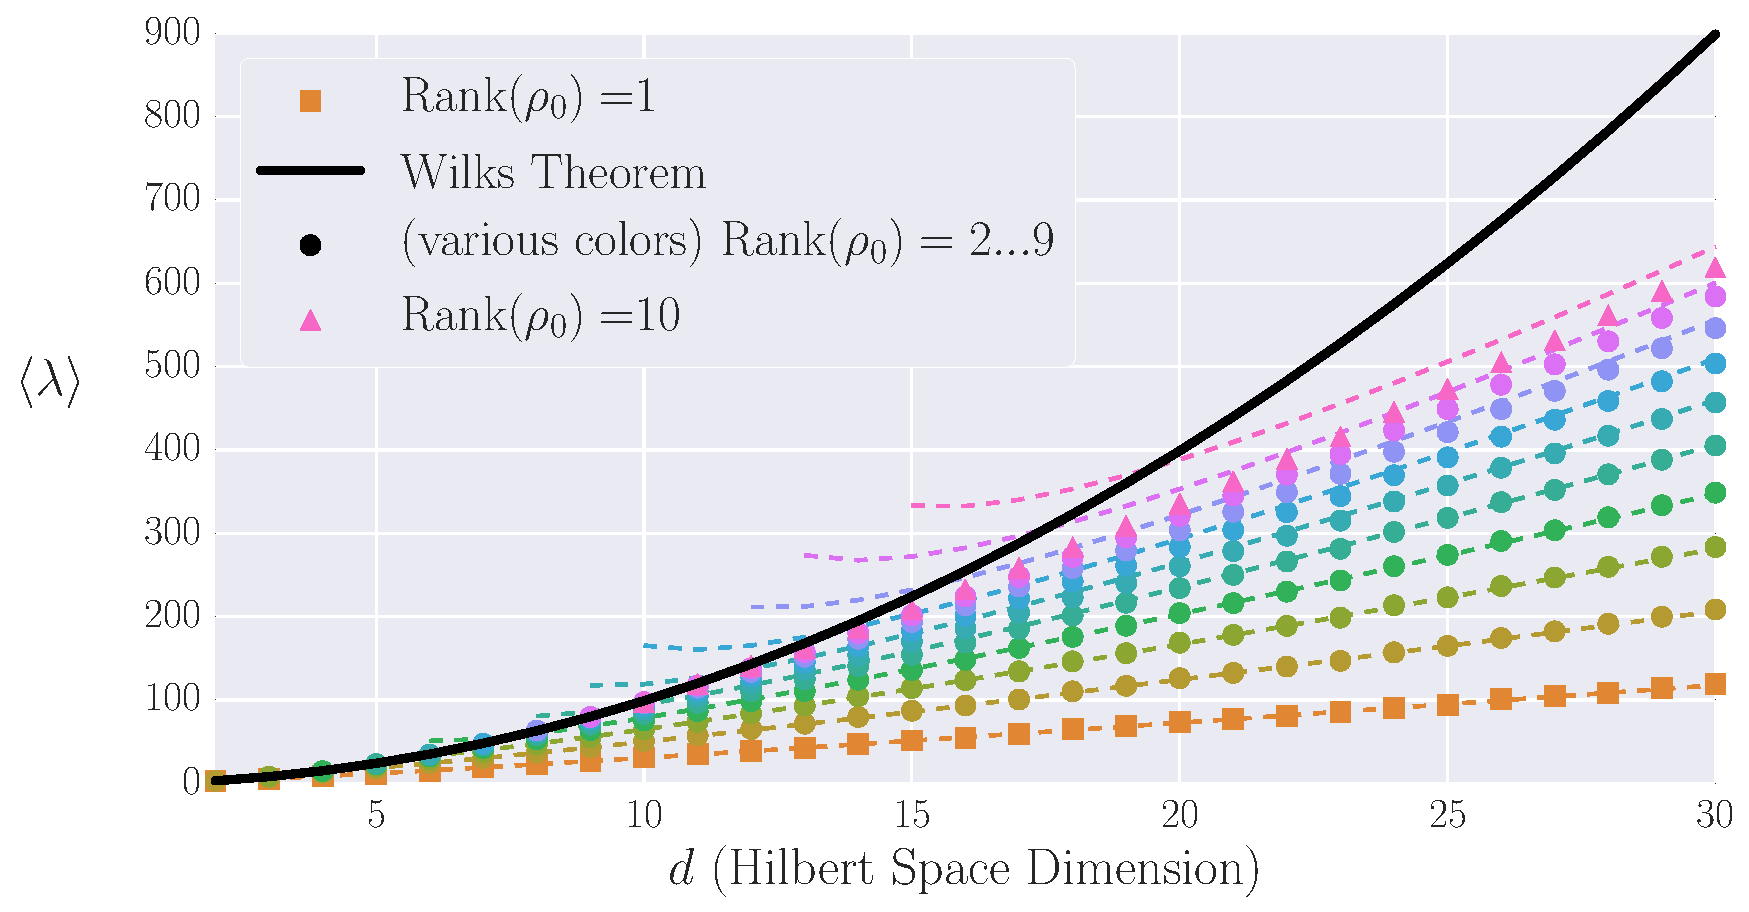
\includegraphics[width=\columnwidth]{Images/Figure_5.pdf}
\caption{Typical samples of GUE($N$) eigenvalues are accurately approximated by order statistics of the distribution (average values of sorted sample).  \textbf{Top}:  The sorted eigenvalues of one randomly chosen GUE(100) matrix.  \textbf{Bottom}:  Approximate values of the order statistics of the GUE(100) distribution, computed as the average of the sorted eigenvalues of 100 randomly chosen GUE(100) matrices.}
\label{fig:orderstatistics1}
\end{figure}

Suppose that $\bvec{\kappa}$ are the eigenvalues of a GUE($N$) matrix, sorted from highest to lowest.  Figure \ref{fig:orderstatistics1} illustrates such a sample for $N=100$.  It also shows the \emph{average} values of 100 such samples (all sorted).  These are the \emph{order statistics} $\overline{\bvec{\kappa}}$ of the distribution (more precisely, what is shown is a good \emph{estimate} of the order statistics; the actual order statistics would be given by the average over infinitely many samples).  The point of the figure is to show that, while the order statistics \emph{are} slightly more smoothly and predictably distributed than a single (sorted) sample\ldots the two are remarkably similar.  A single sample $\bvec{\kappa}$ will fluctuate around the order statistics, but these fluctuations are relatively small, partly because the sample is large, and partly because the GUE eigenvalues experience level repulsion.  Thus, the ``typical'' behavior of a sample -- by which we mean the mean value of a statistic of the sample -- is well captured by the order statistics (which have no fluctuations at all).

We now turn to the problem of modeling $\bvec{\kappa}$ quantitatively.  We note up front that we are only going to be interested in certain properties of $\bvec{\kappa}$:  specifically, partial sums of all $\kappa_j$ greater or less than some threshold (this threshold is $q$ in the main text), or partial sums of functions of the $\kappa_j$ (e.g. $(\kappa_j-q)^2$).  We require only that an ansatz be accurate for such quantities.  We do not use this fact explicitly, but it motivates our approach -- and we do not claim that our ansatz is accurate for \emph{all} conceivable statistics.

In general, if a sample $\bvec{\kappa}$ of size $N$ is drawn so that each $\kappa$ has the same probability distribution 
function $\mathrm{Pr}(\kappa)$, then a good approximation for the $j$th order statistic is given by the inverse 
\emph{cumulative} distribution function (CDF):
\begin{equation}
\overline{\kappa}_j \approx \mathrm{CDF}^{-1}\left(\frac{j-1/2}{N}\right).
\end{equation}
This is closely related to the observation that the histogram of a sample tends to look similar to the underlying probability distribution function.  More precisely, it is equivalent to the observation that the empirical distribution function (the CDF of the histogram) tends to be (even more) similar to the underlying CDF.  (For i.i.d. samples, this is the content of the Glivenko-Cantelli theorem \cite{VanderVaart2000}).  Figure \ref{fig:orderstatistics2} compares the order statistics of GUE(100) and GUE(10) eigenvalues (computed as numerical averages over 100 random samples) to the inverse CDF for the Wigner semicircle distribution.  Even though the Wigner semicircle model of GUE eigenvalues is only exact as $N\to\infty$, it provides a nearly-perfect model for $\overline{\bvec{\kappa}}$ even at $N=10$ (and remains surprisingly good all the way down to $N=2$).

\begin{figure}[h!]
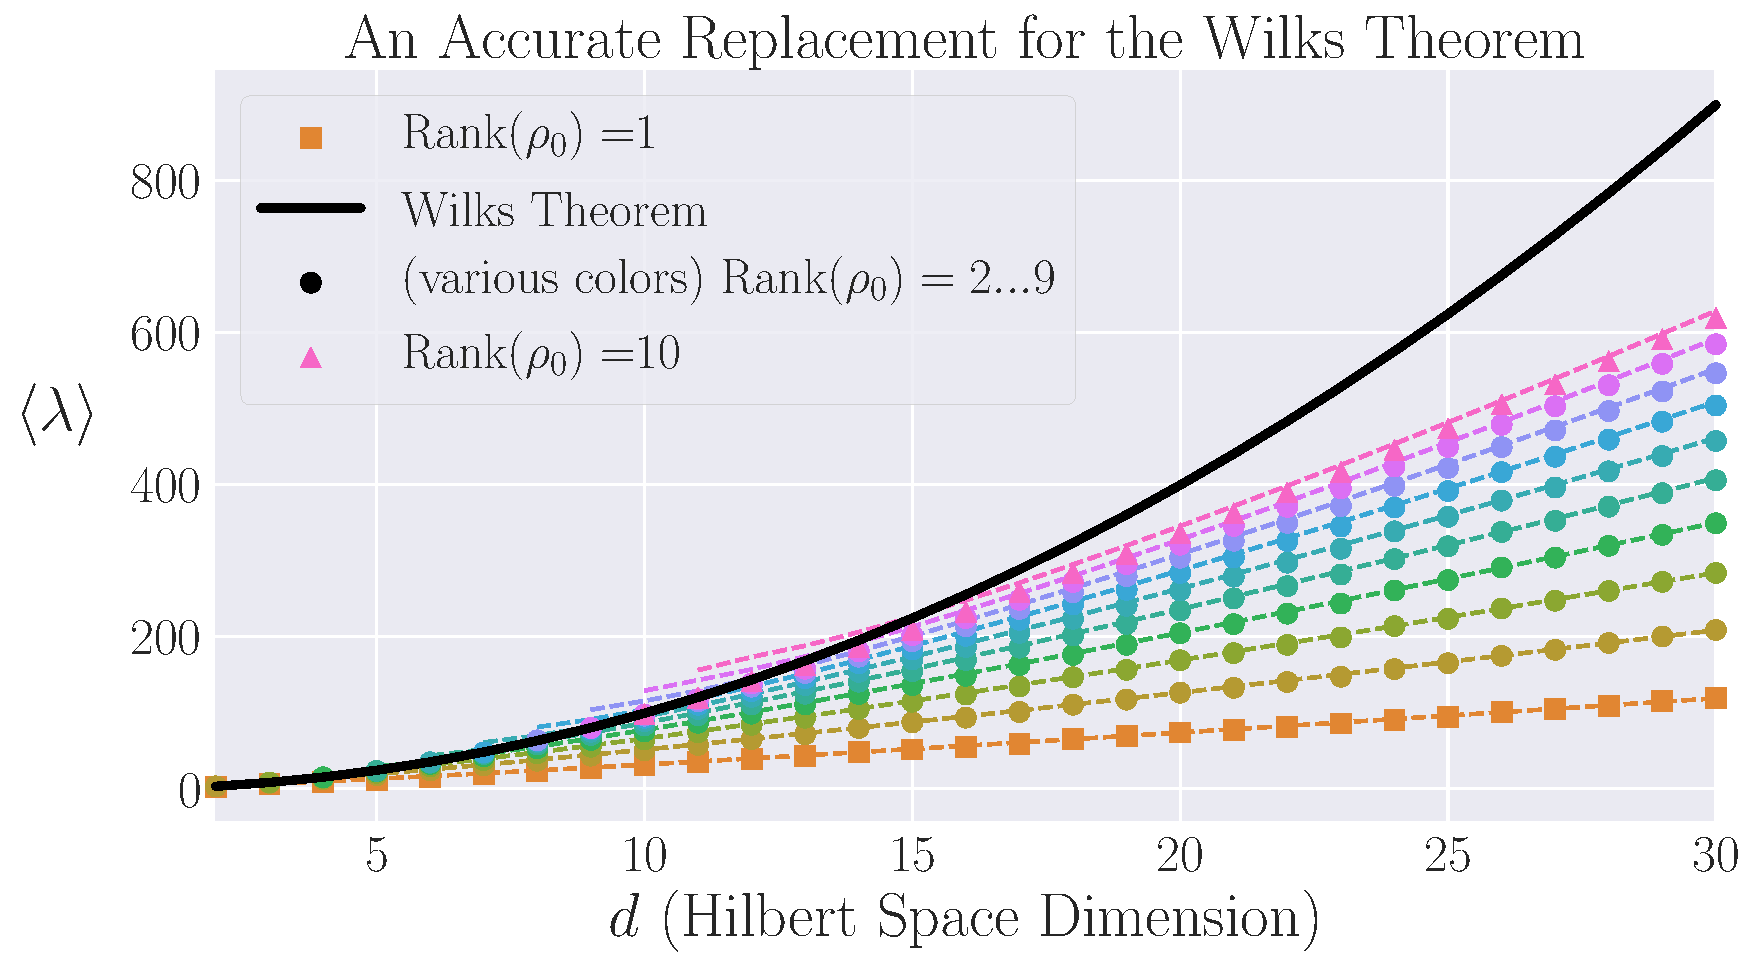
\includegraphics[width=\columnwidth]{Images/Figure_6.pdf}
\caption{Order statistics of the GUE(N) eigenvalue distribution are very well approximated by the inverse CDF of the Wigner semicircle distribution.  \textbf{Top}:  Comparison of the order statistics of the GUE(100) distribution (as shown in Figure \ref{fig:orderstatistics1}) to the inverse CDF of the Wigner semicircle distribution for N=100.  \textbf{Bottom}:  Comparison of the order statistics of the GUE(10) distribution to the inverse CDF of the Wigner semicircle distribution for N=10.  Agreement in both cases is essentially perfect.}
\label{fig:orderstatistics2}
\end{figure}

We make one further approximation, by assuming (as an ansatz) that $N\gg1$, and thus that the distribution of the $\overline{\kappa}_j$ is effectively continuous and identical to $\mathrm{Pr}(\kappa)$. For the quantities that we compute, this is equivalent to replacing the empirical distribution function (which is a step function) by the CDF of the Wigner semicircle distribution.  So, whereas for any given sample the partial sum of all $\kappa_j > q$ jumps discontinuously when $q=\kappa_j$ for any $j$, in this approximation it changes smoothly.  This accurately models the \emph{average} behavior of partial sums.

These approximations provide the ansatz that we use below, for the eigenvalues of $\hat\rho$, as $\{p_j\} \cup \{\overline{\kappa}_j\}$, where the $p_j$ are $\mathcal{N}(\rho_{jj},\epsilon^2)$ random variables, and the $\overline{\kappa}_j$ are the (fixed, smoothed) order statistics of a Wigner semicircle distribution.  

To proceed with truncation, we observe that the $\overline{\kappa}_j$ are symmetrically distributed around $
\kappa=0$, so half of them are negative.  Therefore, with high probability, $\Tr
\left[\mathrm{Trunc}(\hat\rho)\right]>1$, and so we will need to subtract $q\Id$ from $\hat\rho$ before truncating.
Defining $f(q) = \Tr\left[\mathrm{Trunc}(\hat\rho - q \Id)\right]$, the appropriate $q$ solves $f(q) = 1$. Given the assumptions and approximations above, and letting $(x)^{+}$ denote $\mathrm{max}(x,0)$, 
\begin{eqnarray}
\nonumber &&f(q) = \sum_{j=1}^{r}(p_j - q) + \sum_{j=1}^{N}{(\overline{\kappa}_j-q)^+} \\
\nonumber &&\approx 1 - rq + \Delta + N\int_{\kappa=q}^{2\epsilon\sqrt{N}}{(\kappa-q)\mathrm{Pr}(\kappa)\mathrm{d}\kappa}\\
&&= 1 - rq + \Delta + \frac{\epsilon}{12\pi}\left[
\begin{array}{l} (q^2+8N)\sqrt{-q^2+4N} \\
-12qN\left(\frac{\pi}{2}-\sin^{-1}\left(\frac{q}{2\sqrt{N}}\right)\right)
\end{array}\right],\nonumber\\
~
\end{eqnarray}
where $\Delta = \sum_{j=1}^{r}\delta_{jj}$ is a $\mathcal{N}(0,r\epsilon^2)$ random variable.  We also chose to replace a discrete 
sum (line 1) with an integral (line 2).  This approximation is valid when $N\gg1$, where (as noted in the main text) we can accurately approximate a discrete collection of closely spaced real numbers by a smooth density or distribution over the real numbers that has approximately the same CDF.  It is also remarkably accurate in practice.
  
In yet another approximation, we replace $\Delta$ with its average value, which is zero.  We could obtain an even more accurate expression 
 by treating the fluctuations in $\Delta$ more carefully, but this crude approximation turns out to be quite accurate already.

To solve for $f(q) = 1$, it is necessary to further simplify the complicated expression resulting from the integral.  To do so, we 
assume that $\rho_0$ is relatively low-rank, so $r \ll N$.  In this case, the sum of the positive $\overline{\kappa}_j$ is large compared 
with $r$, almost all of them need to be subtracted away, and therefore $q$ is close to $2\epsilon\sqrt{N}$.  We therefore replace 
the complicated expression with its leading order Taylor expansion around $q=2\epsilon\sqrt{N}$, substitute into $f(q)=1$, and 
obtain the equation
\begin{equation}
rq  = \frac{4}{15\pi}N^{1/4}\left(2\sqrt{N}-q\right)^{5/2}.
\end{equation}
This equation is a quintic polynomial, so it has no closed-form solution.  However, its roots have a well-defined asymptotic ($N\to
\infty$) expansion that becomes accurate quite rapidly (e.g., for $N>4$):
\begin{equation}
\label{eq:truncation}
q \approx 2\sqrt{N}-\frac{(240r\pi)^{2/5}}{4}N^{1/10}+\frac{(240r\pi)^{4/5}}{80}N^{-3/10}.
\end{equation}
\todo[inline]{Is it $q/\epsilon$?}
Now that we know how much to subtract off in the truncation process, we can compute $\expect{\lambda}_{\mathrm{kite}}$:
\begin{eqnarray}
\nonumber \expect{\lambda}_{\mathrm{kite}} &=& \left\langle\sum_{j=1}^{r}[\rho_{jj}- (p_j-q)]^2 + \sum_{j=1}^{N}\left[(\kappa_j-q)^+\right]^2 \right\rangle\\
\nonumber  &\approx& r + rq^2 + N\int_{\kappa=q}^{2\epsilon\sqrt{N}}{ Pr(\kappa)(\kappa-q)^2 d\kappa} \\
\nonumber &=& r + rq^2 + \frac{N(N+q^2)}{\pi} \left( \frac{\pi}{2} - \sin^{-1}\left(\frac{q}{2\sqrt{N}}\right)\right)  \nonumber \\
&&\hspace{0.3in}-\frac{q(q^2+26N)}{24\pi} \sqrt{4N-q^2}.
\end{eqnarray}
Thus the total expected value, $\expect{\lambda} = \expect{\lambda}_{\mathrm{L}} + \expect{\lambda}_{\mathrm{kite}}$, is 

\begin{align}
\label{eq:ourLLRS}
\nonumber \langle \lambda(\rho_{0}, \M_{d}) \rangle &\approx 2rd - r^{2}+rq^{2}\\
\nonumber &+  \frac{N(N+q^2)}{\pi} \left( \frac{\pi}{2} - \sin^{-1}\left(\frac{q}{{2\sqrt{N}}}\right)\right)\\
& - \frac{q(q^2+26N)}{24\pi} \sqrt{4N-q^2}
\end{align}
where $q$ is given in Equation \eqref{eq:truncation}, $N=d-r$, and $r = \mathrm{Rank}(\rho_{0})$.

Equation \eqref{eq:ourLLRS} is our main result.  To test its validity, we compare it to numerical simulations for $d=2,\ldots,30$ and $r=1,\ldots,10$, in Figure \ref{fig:modelcomp-iso}.  The prediction of the Wilks Theorem is wildly incorrect for $r\ll d$. In contrast, Equation \ref{eq:ourLLRS} is almost perfectly accurate when $r \ll d$, but it does begin to break down (albeit fairly gracefully) as $r$ becomes comparable to $d$.  We conclude that our analysis [and Equation \eqref{eq:ourLLRS}] correctly models tomography \emph{if} the Fisher information is isotropic ($\Fi \propto \Id$).

\begin{figure}[h]
 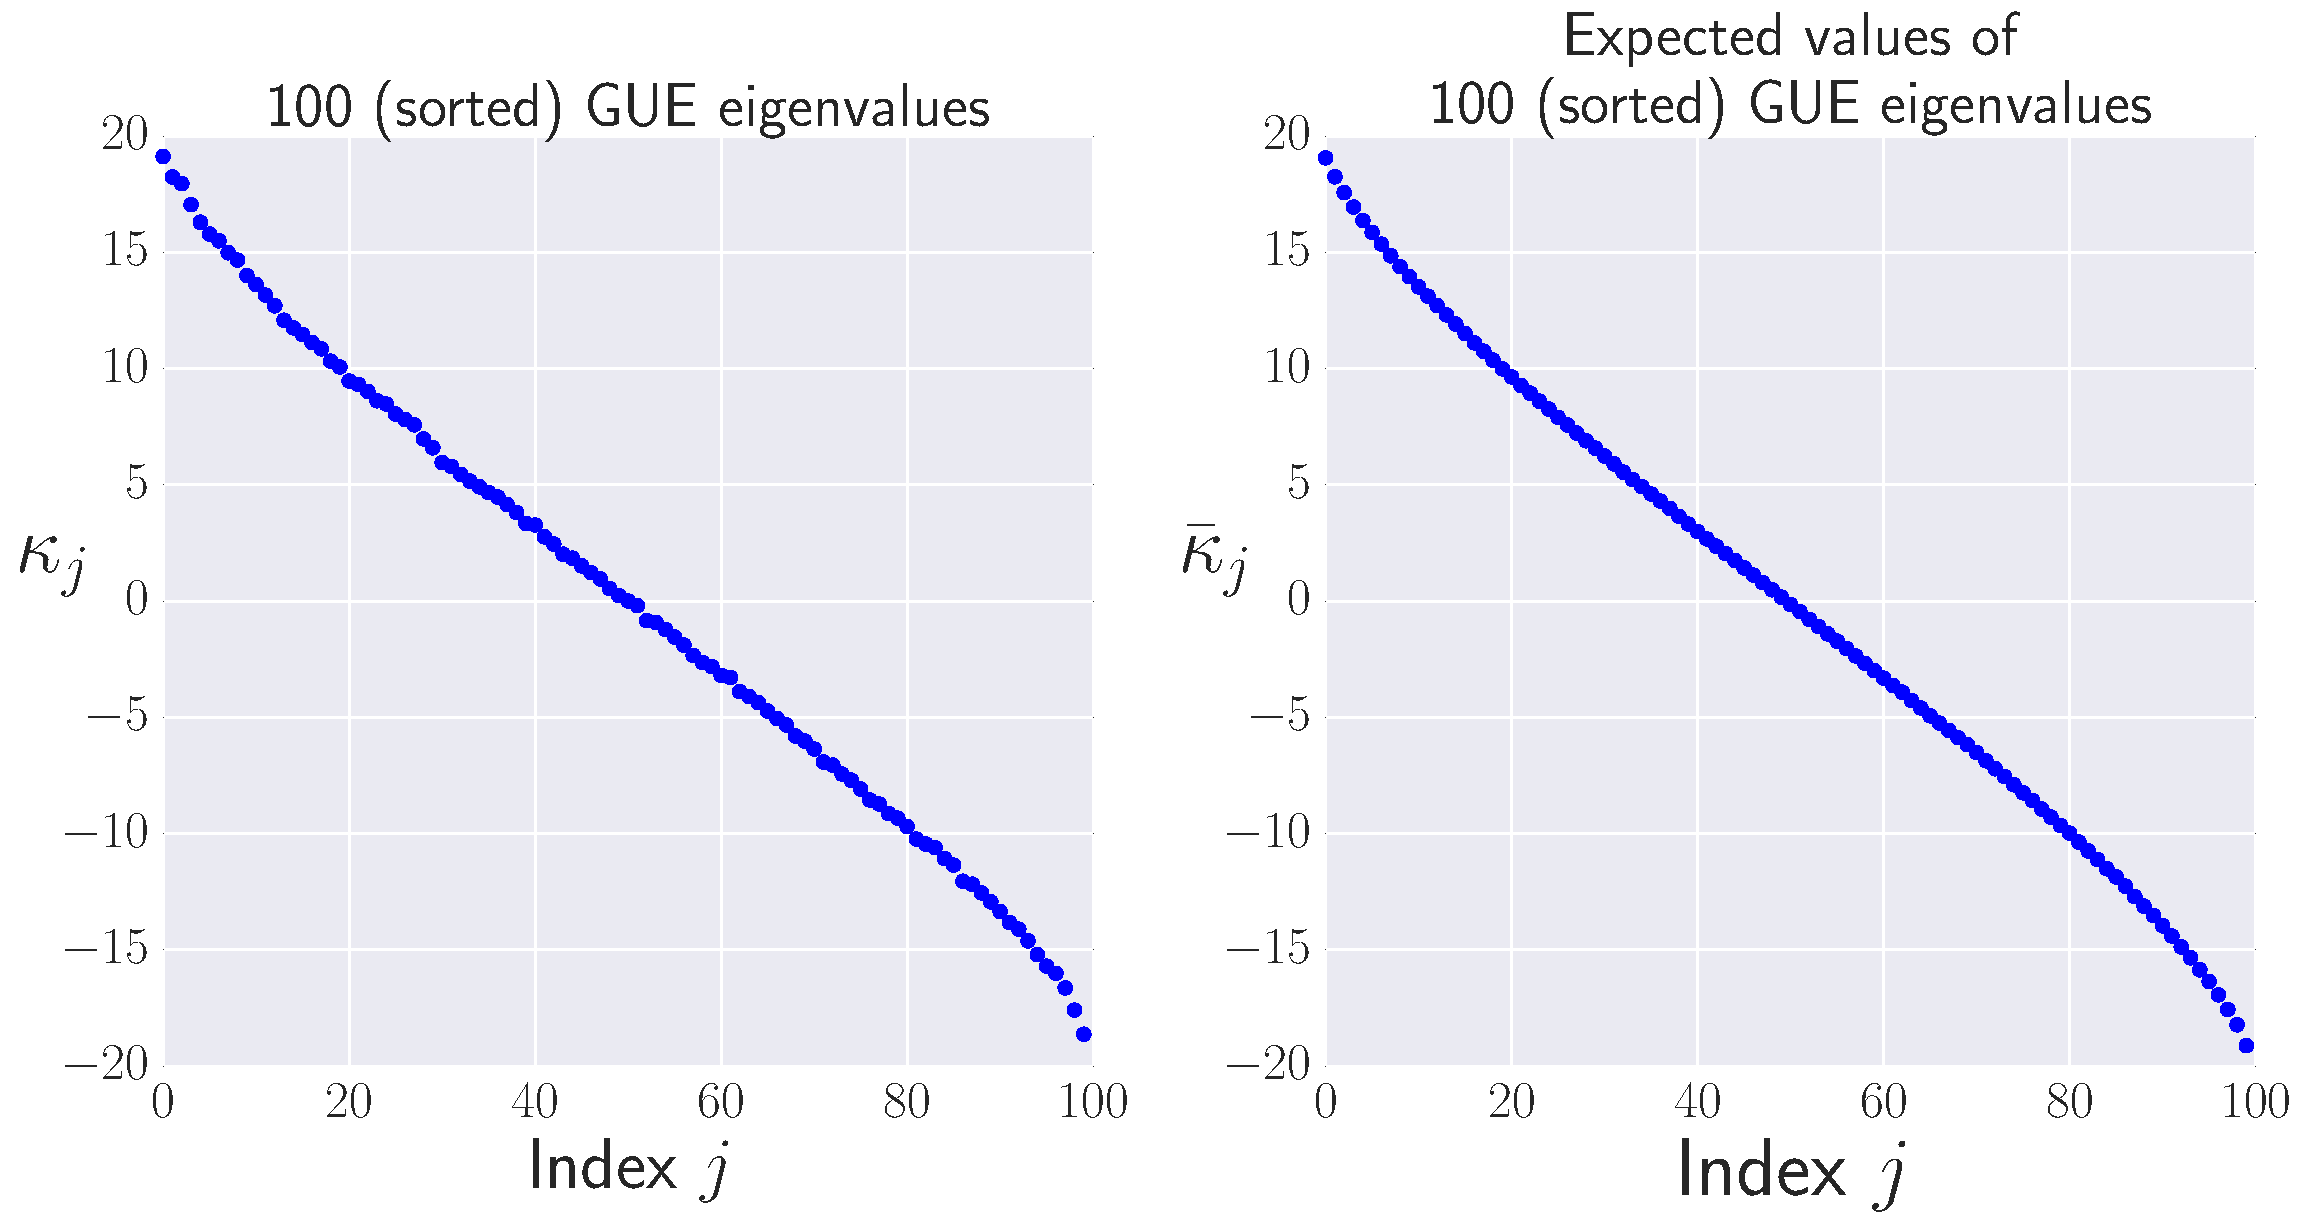
\includegraphics[width=\columnwidth]{Images/Figure_3.pdf}
 \caption{Numerical results for $\expect{\lambda}$ compared to the prediction of the Wilks Theorem (solid line) and our replacement theory as given in Eq. \ref{eq:ourLLRS}, (dashed lines).  Our formula depends on the rank $r$ of $\rho_0$ (unlike the Wilks prediction), and is nearly perfect for $r\ll d$.  It becomes less accurate as $r$ approaches $d/2$, and is invalid when $r\approx d$.}
 \label{fig:modelcomp-iso}
\end{figure}

%----------HETERODYNE TOMOGRAPHY-----------%
In practice, the Fisher information is rarely isotropic.  So we tested our idealized result by applying it to a realistic, challenging, and experimentally relevant problem: quantum heterodyne (equivalent to double homodyne) state tomography \cite{Lvovsky2001a, Bertrand1987, Leonhardt1995, Lvovsky2009} of a single optical mode.  (See Figure \ref{fig:fish_condition} for a plot of the \emph{condition number} -- the ratio of the largest to smallest eigenvalue -- of the estimated Fisher information. It is clear that, for such a tomographic setup, $\mathcal{I} \not \propto \Id$.) States of this continuous-variable system are described by density operators on the infinite-dimensional Hilbert space $L^2(\reals)$.  Fitting these infinitely many parameters to finitely much data demands simpler models.
We consider a family of nested models motivated by a low-energy (few-photon) ansatz, and choose   
the Hilbert space $\mathcal{H}_d$ to be that spanned by the photon number states $\{\ket{0}\ldots\ket{d-1}\}$.
Heterodyne tomography reconstructs $\rho_{0}$ using data from repeated measurements of the 
coherent-state POVM, $\{|\alpha\rangle\langle \alpha| /\pi, ~\alpha=x+ip\in \mathbb{C}\}$, which corresponds to sampling directly from the 
state's Husimi $Q$-function \cite{Husimi1940}.

\begin{figure}[h]
  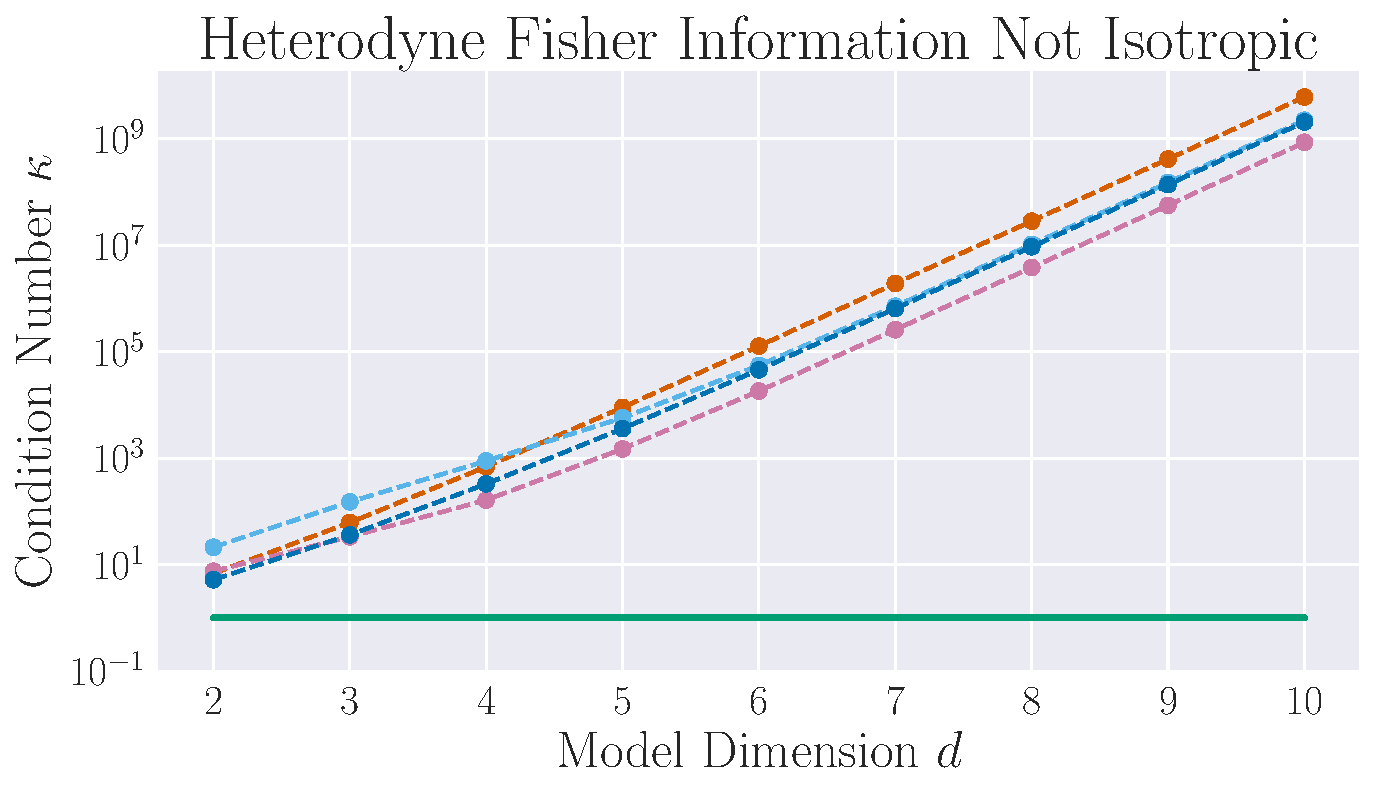
\includegraphics[width=\columnwidth]{Images/Figure_10.pdf}
 \caption{The condition number $\kappa$ -- the ratio of the largest to smallest eigenvalue -- of the estimated Fisher information grows with model dimension, indicating an increase in anisotropy. (Estimates are the average over 100 Hessians of the loglikelihood function.) The dashed lines indicate different true states $\rho_{0}$, and the solid line is $\kappa = 1$ (i.e., $\mathcal{I} \propto \Id$.).}
\label{fig:fish_condition}
\end{figure}

We examined the behavior of $\lambda$ for 13 distinct true states $\rho_{0}$, both pure and mixed, supported on $\mathcal{H}_{2}, \mathcal{H}_{3}, \mathcal{H}
_{4}$, and $\mathcal{H}_{5}$.  We used rejection sampling to simulate 100 heterodyne datasets with up to $N_{\mathrm{samples}}=10^5$, and found MLEs over each of the 9 models $\M_2, \ldots, M_{10}$ using numerical optimization \footnote{The model $\M_{1}$ is trivial, as $\M_{1} = \{|0\rangle \langle 0|\}$. This model will almost always be wrong, in general.}.  For each true state and each $d$, we averaged $\lambda(\rho_{0}, \M_{d})$ over all 100 datasets to obtain an empirical average loglikelihood ratio $\bar{\lambda}$ for each $(\rho_0,d)$ pair.

\begin{figure}[h]
 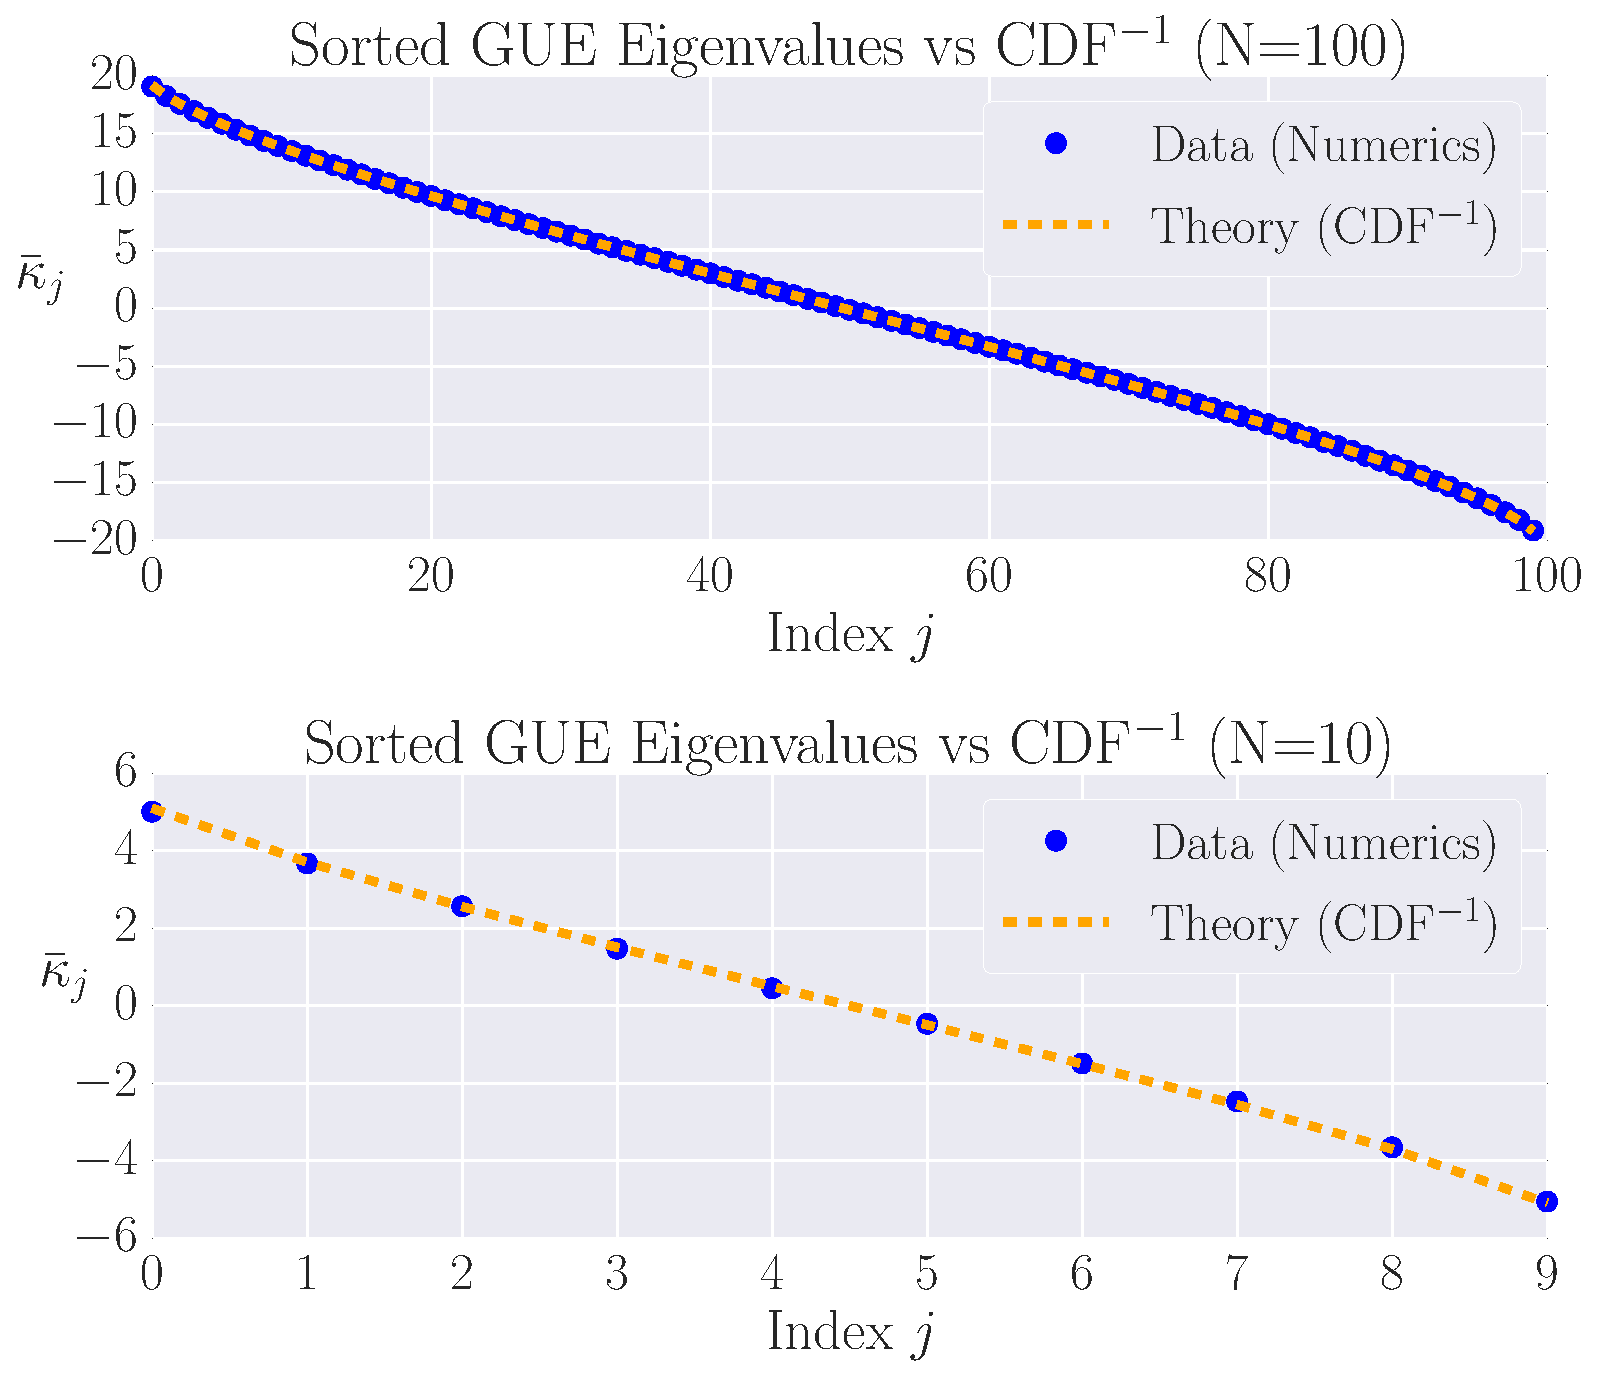
\includegraphics[width=\columnwidth]{Images/Figure_4.pdf}
 \caption{The Wilks Theorem (orange dots) dramatically over-estimates $\langle\lambda(\rho_{0}, \M_{d})\rangle$ in optical heterodyne tomography. Our formula, Equation \ref{eq:ourLLRS} (blue squares), is far more accurate. Residual discrepancies, discussed in Appendix \ref{app:breakdown}, appear to stem largely from non-asymptoticity ($N_{\mathrm{samples}}$ is not yet ``asymptotically large''). The solid red line of equality corresponds to perfect correlation between theory ($\expect{\lambda}$) and practice ($\bar\lambda$).}
 \label{fig:modelcomp}
\end{figure}

Results of this test are shown in Figure \ref{fig:modelcomp}, where we plot (a) the Wilks prediction, and (b) Equation \eqref{eq:ourLLRS}, against the empirical $\bar\lambda$, for a variety of true states and reconstruction dimensions.  Our formula correlates very well with the empirical average, while the Wilks Theorem (unsurprisingly) overestimates $\lambda$ dramatically for low-rank states.  Whereas a model selection procedure based on Wilks Theorem would tend to falsely reject larger Hilbert spaces (by setting the threshold for acceptance too high), our formula provides a reliable null theory.

Interestingly, as $d$ grows, Equation \eqref{eq:ourLLRS} also begins to overpredict.  Further investigation (see Appendix \ref{app:breakdown}) indicates that a more accurate description is that the numerical experiments are \emph{underachieving}, because $N_{\mathrm{samples}}$ is not large enough -- $\bar\lambda$ is still growing with $N_{\mathrm{samples}}$.  Our analysis is explicitly asymptotic, and does not cover this case.  Failing to reach asymptotic behavior at $N_{\mathrm{samples}}=10^5$ is surprising, and suggests that heterodyne tomography is a particular exceptional and challenging case to model statistically.

%--------CONCLUSIONS----------%
The Wilks Theorem is not generally reliable in quantum state tomography, but our Equation \eqref{eq:ourLLRS} provides a much more broadly applicable replacement that can be used in model selection methods.  This includes protocols like the AIC and BIC \cite{Akaike1974, Schwarz1978, Burnham2004} that do not explicitly use the Wilks Theorem, but rely on the same assumptions (asymptotic normality, etc).  Null theories of the loglikelihood ratios have many other applications, including hypothesis testing \cite{Blume-Kohout2010,Moroder2013} and confidence regions \cite{Glancy2012a}, and our result is directly applicable to them.  Refs. \cite{Moroder2013,Glancy2012a} both point out explicitly that their methods are unreliable near boundaries and therefore cannot be applied to rank-deficient states; our result fixes this outstanding problem.  However, our numerical experiments with heterodyne tomography show unexpected behavior, indicating that quantum tomography can still surprise, and may violate \emph{all} asymptotic statistics results.  In such cases, bootstrapping \cite{Efron1979} may be the only reliable way to construct null theories for $\lambda$.  Finally, the \emph{methods} presented here have application beyond the analysis of loglikelihoods.  They shed light on the behavior of $\rhoMLE$ for rank-deficient states, and can be used to predict other derived properties such as the average rank of the estimate, which is independently interesting for (e.g.) quantum compressed sensing \cite{Flammia2012a, Kalev2015, Kalev2015a}.

\noindent\textbf{Acknowledgements:} The authors are grateful for those who provide support for the following software packages: iPython/Jupyter \cite{Perez}, matplotlib
\cite{Hunter2007}, mpi4py \cite{Dalcin2005},  NumPy \cite{VanDerWalt2011}, pandas \cite{mckinney2010}, Python 2.7 
\cite{vanRossum}, seaborn \cite{Waskom2016}, and SciPy \cite{Oliphant2007a}. TLS thanks Jonathan A Gross for helpful 
discussions on software design, coding, and statistics, John King Gamble for useful insights on parallelized 
computation and feedback on earlier drafts of this paper, and Daniel Seuss for proofreading edits.

Sandia National Laboratories is a multi-mission laboratory managed and operated by Sandia Corporation, a wholly owned 
subsidiary of Lockheed Martin Corporation, for the U.S. Department of Energy's National Nuclear Security Administration 
under contract DE-AC04-94AL85000.

\bibliographystyle{apsrev}
\bibliography{wilkspaper}

\newpage
\newpage

%---------------------------APPENDICES------------------------------%
\begin{center}\textbf{SUPPLEMENTAL MATERIAL}\end{center}

%-----------DERIVATION OF WILKS REPLACEMENT DETAILS-----------%
\section{Derivation of the Wilks replacement: technical details}
\label{app:technical}







\begin{figure}[h!]
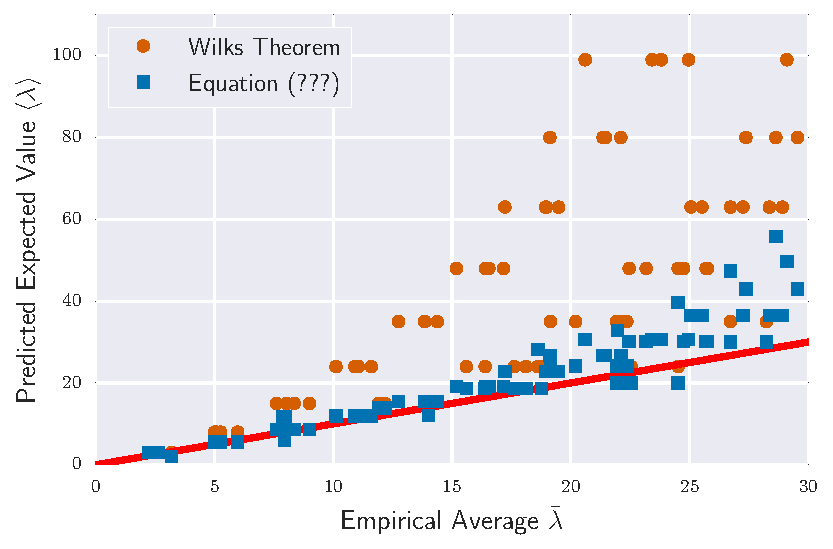
\includegraphics[width=\columnwidth]{Images/Figure_7.pdf}
 \caption{Contributions of each matrix element of $\rhoMLE$ to $\expect{\lambda}$, for three different $\rho_0$, as computed in numerical simulations for $d=8$.  \textbf{Left}:  The matrix elements of $\rho_0$.  \textbf{Right}:  The average scaled mean-squared-errors of individual matrix elements, $\expect{\lambda_{jk}}$, as defined in Eq. 6.  \textbf{Discussion}:  While the Wilks Theorem predicts that each matrix element should contribute $\approx1$, only those in the ``L'' (see Fig. 3) do so; those in the ``kite'' behave quite differently and (generally) contribute less to $\expect{\lambda}$.
}
\label{fig:isocontribs}
\end{figure}



%--------------------MORE ABOUT HETERODYNE TOMOGRAPHY----------------%
\section{Breakdown of Our Model In the Case of Heterodyne Tomography}
\label{app:breakdown}


\begin{figure}[h!]
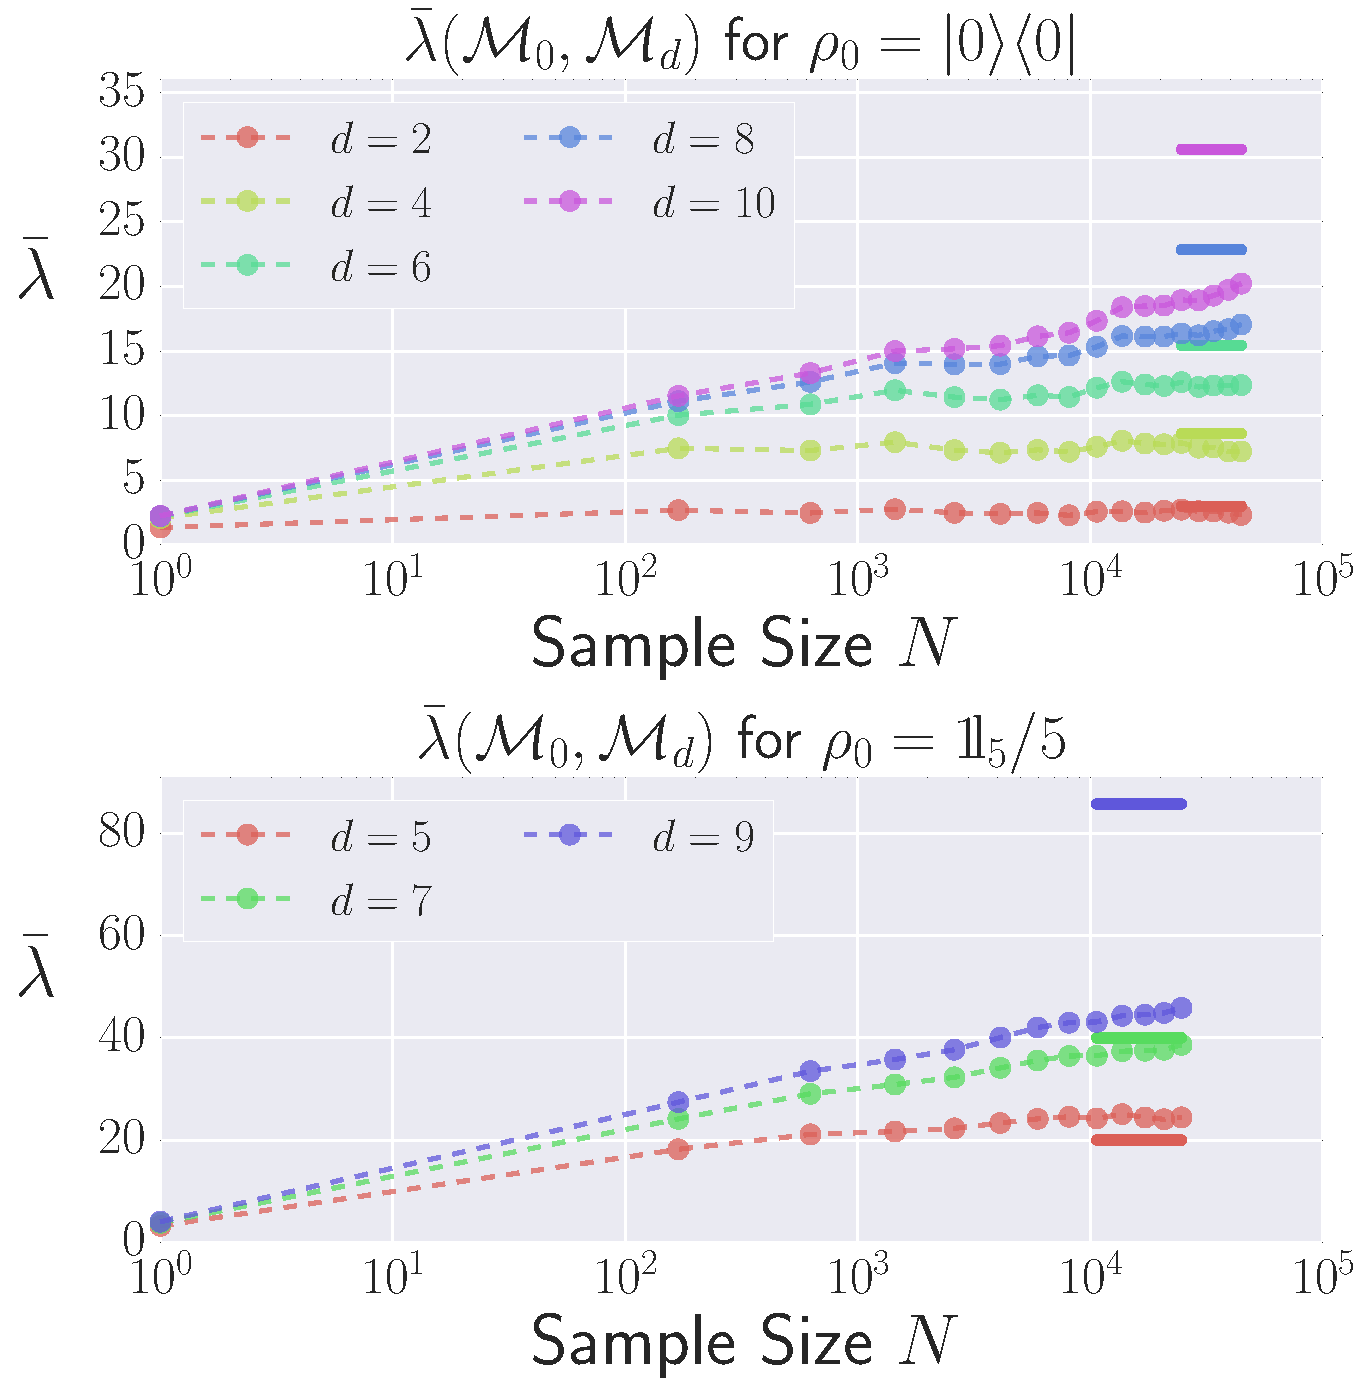
\includegraphics[width=\columnwidth]{Images/Figure_8.pdf}
 \caption{Preliminary results comparing our theory (Equation. \ref{eq:ourLLRS}) and the Wilks Theorem to the empirical expectation value of $\lambda$ for heterodyne tomography with additional $(\rho_{0}, d)$ pairs than shown in Figure \ref{fig:modelcomp}.  For these larger Hilbert space dimensions, our theory begins to fail, for several reasons that we detail in this section.  Most importantly, even at $N=10^5$ samples, we observe (see Figure \ref{fig:totalcontrib}) that the empirical $\lambda$ has not yet asymptoted -- it is still increasing (very slowly) with $N$.  Thus, simulations of heterodyne tomography at the $N$ values considered so far \emph{underperform} our theory.  We conjecture that our theory will become more and more accurate as $N\to\infty$, but that (because certain important events are very, very rare), this convergence will only occur at very large $N = e^{\mathcal{O}(d)}$.  A secondary effect is the anisotropy of the Fisher information (see Figure \ref{fig:fish_condition}), which causes smaller but significant deviations from our theory.}
\label{fig:modelcomp2}
\end{figure}
Although Figure \ref{fig:modelcomp} in the main text shows reasonable agreement between our expression for $\langle \lambda \rangle$ and the numerically computed average $\bar{\lambda}$, the discrepancies are sufficiently large that it behooves us to examine why this may be the case. In this section, we show how finite-sample effects, anisotropy of the Fisher information, and the behavior of the loglikelihood ratio statistic for Poisson-distributed data could explain some of the discrepancy we see in preliminary results for reconstructions with higher dimension $d$ (see Figure \ref{fig:modelcomp2}).

We start by plotting $\bar{\lambda}$ as a function of the number of heterodyne counts $N$. (We did not do any binning of our rejection sampling outcomes, so that each POVM effect is observed only once.) Both the Wilks 
Theorem and our result are derived in an asymptotic limit $N \rightarrow \infty$; for finite but large $N$, our results may be invalid. 
As seen in Figure \ref{fig:totalcontrib}, $\bar{\lambda}$ may be growing, even for $N \sim 10^{5}$, depending on $\rho_{0}$ and $d$.
\begin{figure}[h]
  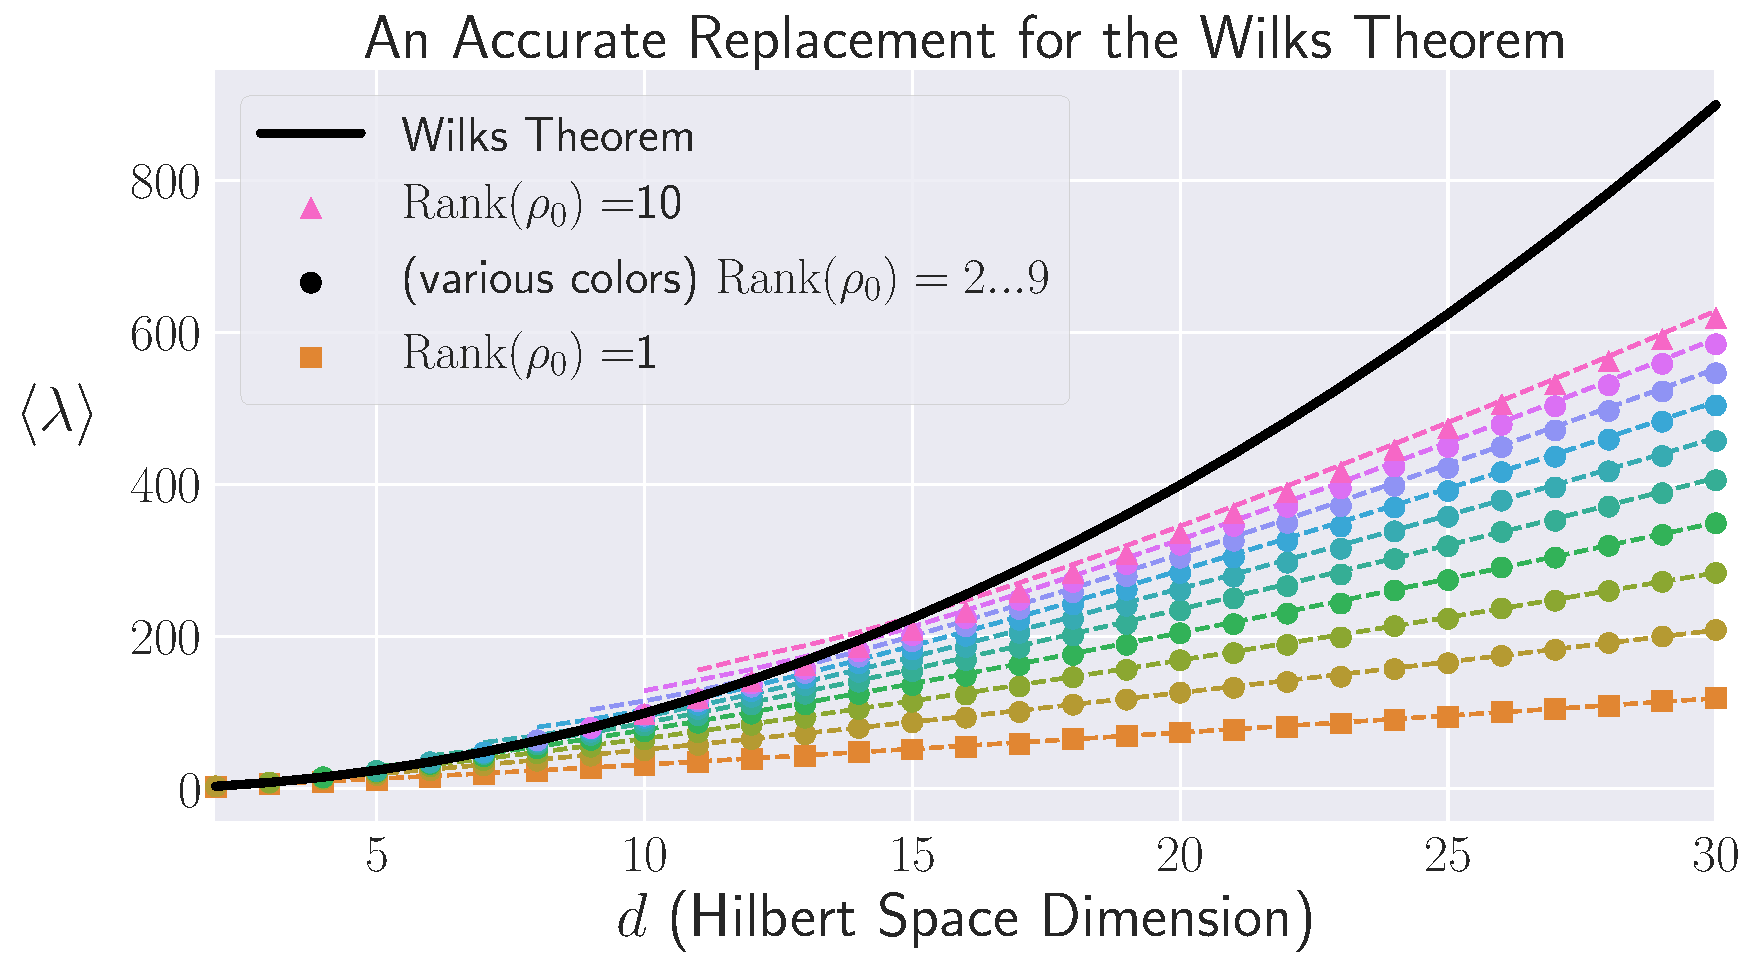
\includegraphics[width=\columnwidth]{Images/Figure_9.pdf}
 \caption{The empirical average $\bar{\lambda}$  may have achieved its asymptotic value, or is still 
growing, depending on the true state $\rho_{0}$ and the model dimension $d$. Solid lines indicate the value of our formula
for the asymptotic expected value, given in Equation \eqref{eq:ourLLRS}.}
\label{fig:totalcontrib}
\end{figure}

Thus, part of the discrepancy between our expression and the numerical results is simply a finite-sample effect. Next, we check 
whether the Fisher information is actually isotropic - a key ingredient in our derivation. To estimate the Fisher information, we use a numerical average of 100 observed informations (Hessians of the loglikelihood function), $\bar{H}$. In  Figure \ref{fig:fish_condition}, we plot, for several $\bar{H}$, their condition number $\kappa$, which is the ratio of the largest eigenvalue to the smallest. Importantly, $\kappa = 1$ if, and only if, all the eigenvalues are the same (i.e., the Fisher information is isotropic). The condition number appears to grow with $d$, meaning the anisotropy is becoming more severe.



If the anisotropy is so severe, why is our model reasonably accurate? To answer this question, we compute the scaled mean squared errors $\langle \lambda_{jk}\rangle$ (defined in Equation \eqref{eq:llrserrors}) for the heterodyne estimates, and compare them to those of our model. As shown in Figure \ref{fig:model_comparison}, we see qualitative agreement - matrix elements in the coherent ``L" contribute about 1 unit of 
expected value, while matrix elements in the ``kite" contribute less than our model predicts.

Looking at each $\langle \lambda_{jk} \rangle$ as a function of the sample size $N$ and $(j, k)$, we see in Figure \ref{fig:individcontrib} that each contribution grows 
starting from zero, and some elements (notably those in the ``L") rapidly achieve their asymptotic 
contribution of ~1.  Those within the ``kite", however, grow much more slowly. Further, the anisotropic nature of the Fisher information may be such that the ``kite" elements will never attain the values predicted by our theory.

Finally, we conjecture, based on strong theoretical support from an an analysis  of the loglikelihood ratio statistic for classical Poisson distributions (Appendix \ref{app:poisson}) that certain matrix elements --- namely, those in the coherent ``L" with support on higher-energy photon states $|n\rangle$ --- do not reach their asymptotic contribution level until  \emph{extremely} large 
sample sizes $N$.  If this conjecture is true, then at least some of our model's failure to match the observed values occurs 
simply because the empirical datasets are not yet ``asymptotically" large, meaning individual $\langle \lambda_{jk}\rangle$ are not yet asymptotic, causing $\langle \lambda \rangle $ to not have achieved its asymptotic value either.

\begin{figure}[h]
  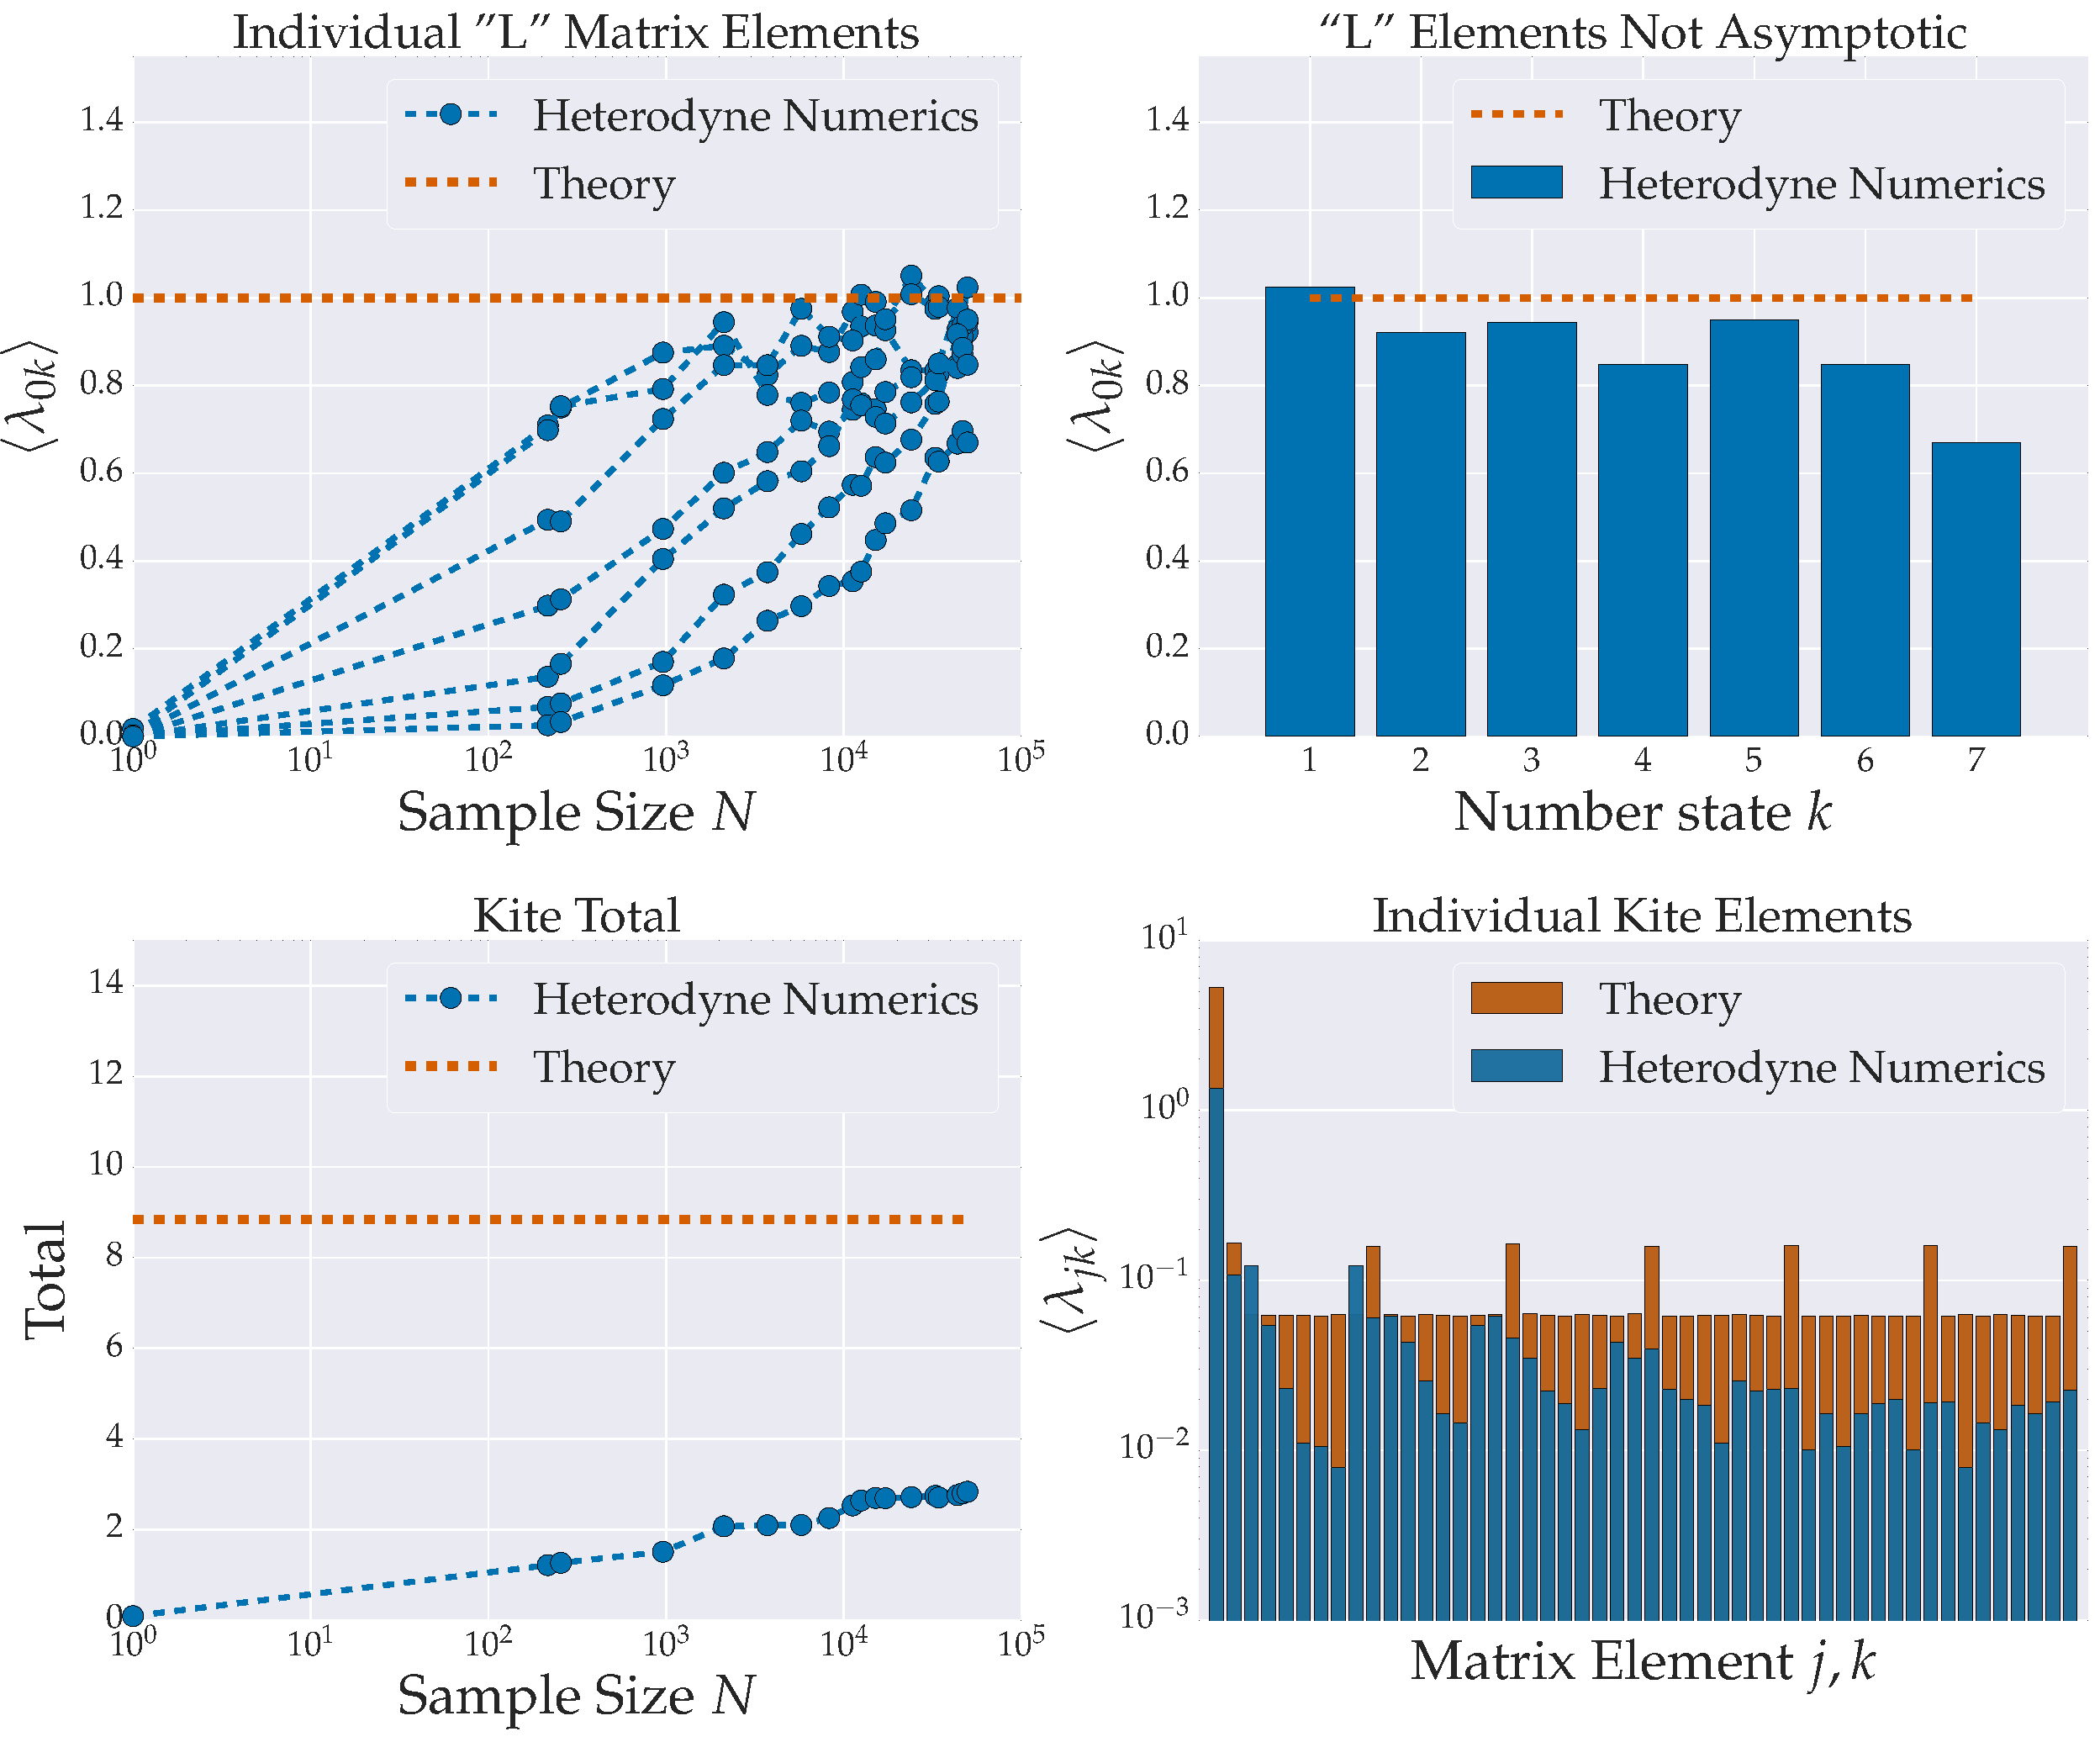
\includegraphics[width=\columnwidth]{Images/Figure_11.pdf}
 \caption{The scaled mean squared errors $\langle \lambda_{jk} \rangle$ assuming an isotropic Fisher information (left), and for heterodyne tomography (right). \textbf{Top}: $\rho_{0} = |0\rangle\langle 0|$. \textbf{Bottom}: $\rho_{0} = \mathcal{I}_{2}/2$. Qualitatively, the behavior of the contributions is the same, though there are quantitative differences, particularly within the
kite.}
\label{fig:model_comparison}
\end{figure}


\begin{figure}[h]
  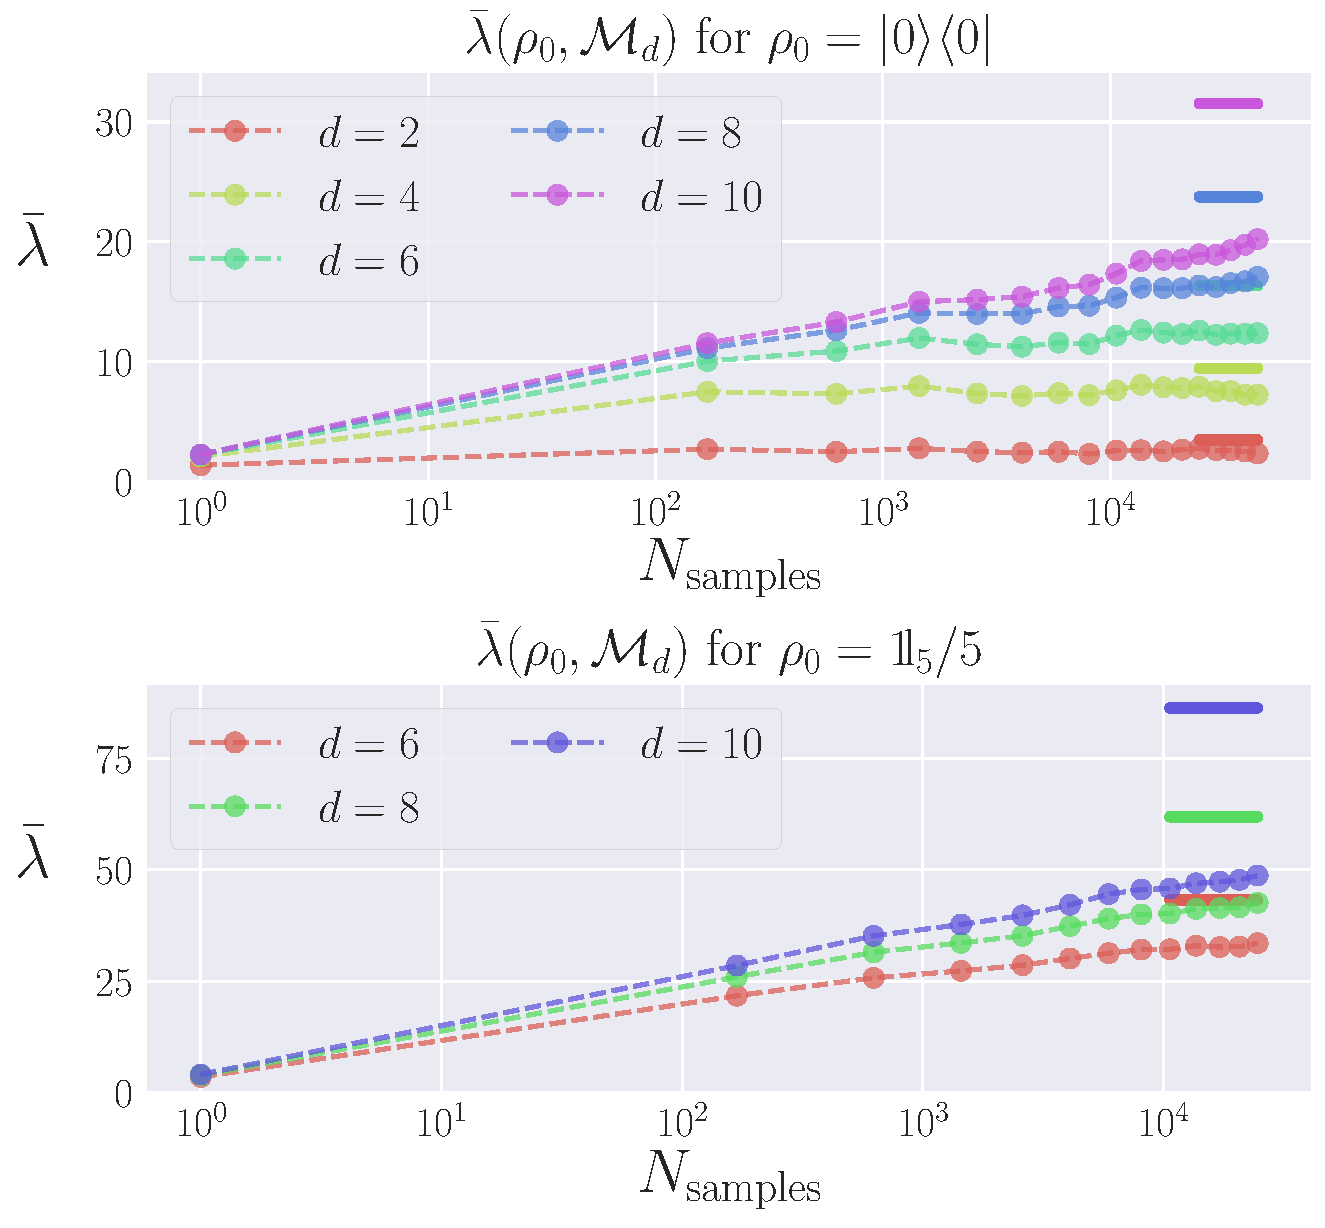
\includegraphics[width=\columnwidth]{Images/Figure_12.pdf}
 \caption{Examining how our predicted values for $\langle \lambda_{jk} \rangle$ disagree with simulated heterodyne experiments. We take $\rho_{0} = |0\rangle\langle 0|$ and $d=8$. \textbf{Top Left}: The fluctuations in the ``L" $\langle \lambda_{0k}\rangle$ as a function of sample size $N$.  \textbf{Top Right}: At the largest $N$ studied, the fluctuations in the ``L" from coherences with different number states. For the higher number states, $\langle \lambda_{0k}\rangle$ is substantially less than 1. \textbf{Bottom Left}: The total from the ``kite" versus $N$. It is clear the total is still growing. \textbf{Bottom Right}: The individual ``kite" elements $\langle \lambda_{jk}\rangle$ at the largest $N$ studied;  most are small compared to the model.}
\label{fig:individcontrib}
\end{figure}



%----------POISSON DIP/BUMP PHENOMENON----------%
\section{The Poisson Bump Phenomenon}
\label{app:poisson}

Here we show how $\langle \lambda \rangle$ depends strongly on the expected number of counts for Poisson-distributed data.
Suppose we are given count data which is Poisson distributed, so that the probability of observing $K$ counts is
\begin{equation}
\mathrm{Pr}(K) = \frac{e^{-\theta_{0}}\theta_{0}^{K}}{K!}
\end{equation}
where $\langle K \rangle = \theta_{0}$. Suppose further we observed 
$C$ counts. The likelihood function is simply
\begin{equation}
\label{eq:poisl}
\cL(\theta) = \mathrm{Pr}(C|\theta) = \frac{e^{-\theta}\theta^{C}}{C!}
\end{equation}
We will compare the models
\[\M_{0}: \theta = \theta_{0}~~~~\M_{1}: \theta \in [0, \infty)\]
using the loglikelihood ratio statistic. By definition, we have
\begin{equation}
\lambda(\M_{0}, \M_{1}) = -2 \log \left(\frac{\mathcal{L}(\theta_{0})}{\mathcal{L}(\hat{\theta})}\right)
\end{equation}
with $\hat{\theta}$ as the MLE of the likelihood function in Equation \eqref{eq:poisl}. Doing the maximization, we find $\hat{\theta} = C$.
Plugging in the MLE yields
\begin{align}
\nonumber \lambda(\M_{0}, \M_{1}) &= -2 \log \left(e^{C-\theta_{0}}\left(\frac{\theta_{0}}{C}\right)^{C}\right)\\
&= -2 \left(C - \theta_{0} + C \log(\theta_{0}) - C \log (C)\right)
\end{align}
According to the Wilks Theorem, $\lambda \sim \chi^{2}_{1}$, since $\M_{1}$ is a one-dimensional model. Accordingly, $\langle 
\lambda \rangle = 1$. Let's compute $\langle \lambda \rangle$ using the expression above:
\begin{equation}
\langle \lambda \rangle = -2 ( \langle C \rangle - \theta_{0} + \langle C \rangle \log(\theta_{0}) - \langle C \log (C)\rangle)
\end{equation}
Using the fact $\langle C \rangle = \theta_{0}$, the above equation simplifies some:
\begin{equation}
\label{eq:pois1}
\langle \lambda \rangle = -2 ( \theta_{0} \log(\theta_{0}) - \langle C \log (C)\rangle)
\end{equation}
We compute the expected value of $C\log(C)$ as
\begin{align*}
\langle C \log(C) \rangle &= \sum_{C=0}^{\infty}C \log (C) \mathrm{Pr}(C) = \sum_{C=0}^{\infty}C \log(C) \frac{e^{-\theta_{0}}
\theta_{0}^{C}}{C!}\\
&= \theta_{0}e^{-\theta_{0}}\sum_{C=0}^{\infty}\frac{\log (C + 1) \theta_{0}^{C}}{C!}
\end{align*}
(In general, for a random variable $X$, $\langle f(X)\rangle \neq f(\langle X \rangle)$, unless $f$ is \emph{linear}.)
Putting this expression into Equation \eqref{eq:pois1} gives
\begin{equation}
\label{eq:pois2}
\langle \lambda \rangle = -2 \left( \theta_{0} \log(\theta_{0}) - \theta_{0}e^{-\theta_{0}}\sum_{C=0}^{\infty}\frac{\log (C + 1) 
\theta_{0}^{C}}{C!}\right)
\end{equation}

In Figure \ref{fig:poissonbump}, we plot $\langle \lambda \rangle$ as a function of $\theta_{0}$, where we truncate the sum at 150 
terms. It is clear $\langle \lambda \rangle$ 
depends strongly on $\theta_{0}$.
\begin{figure}[ht]
  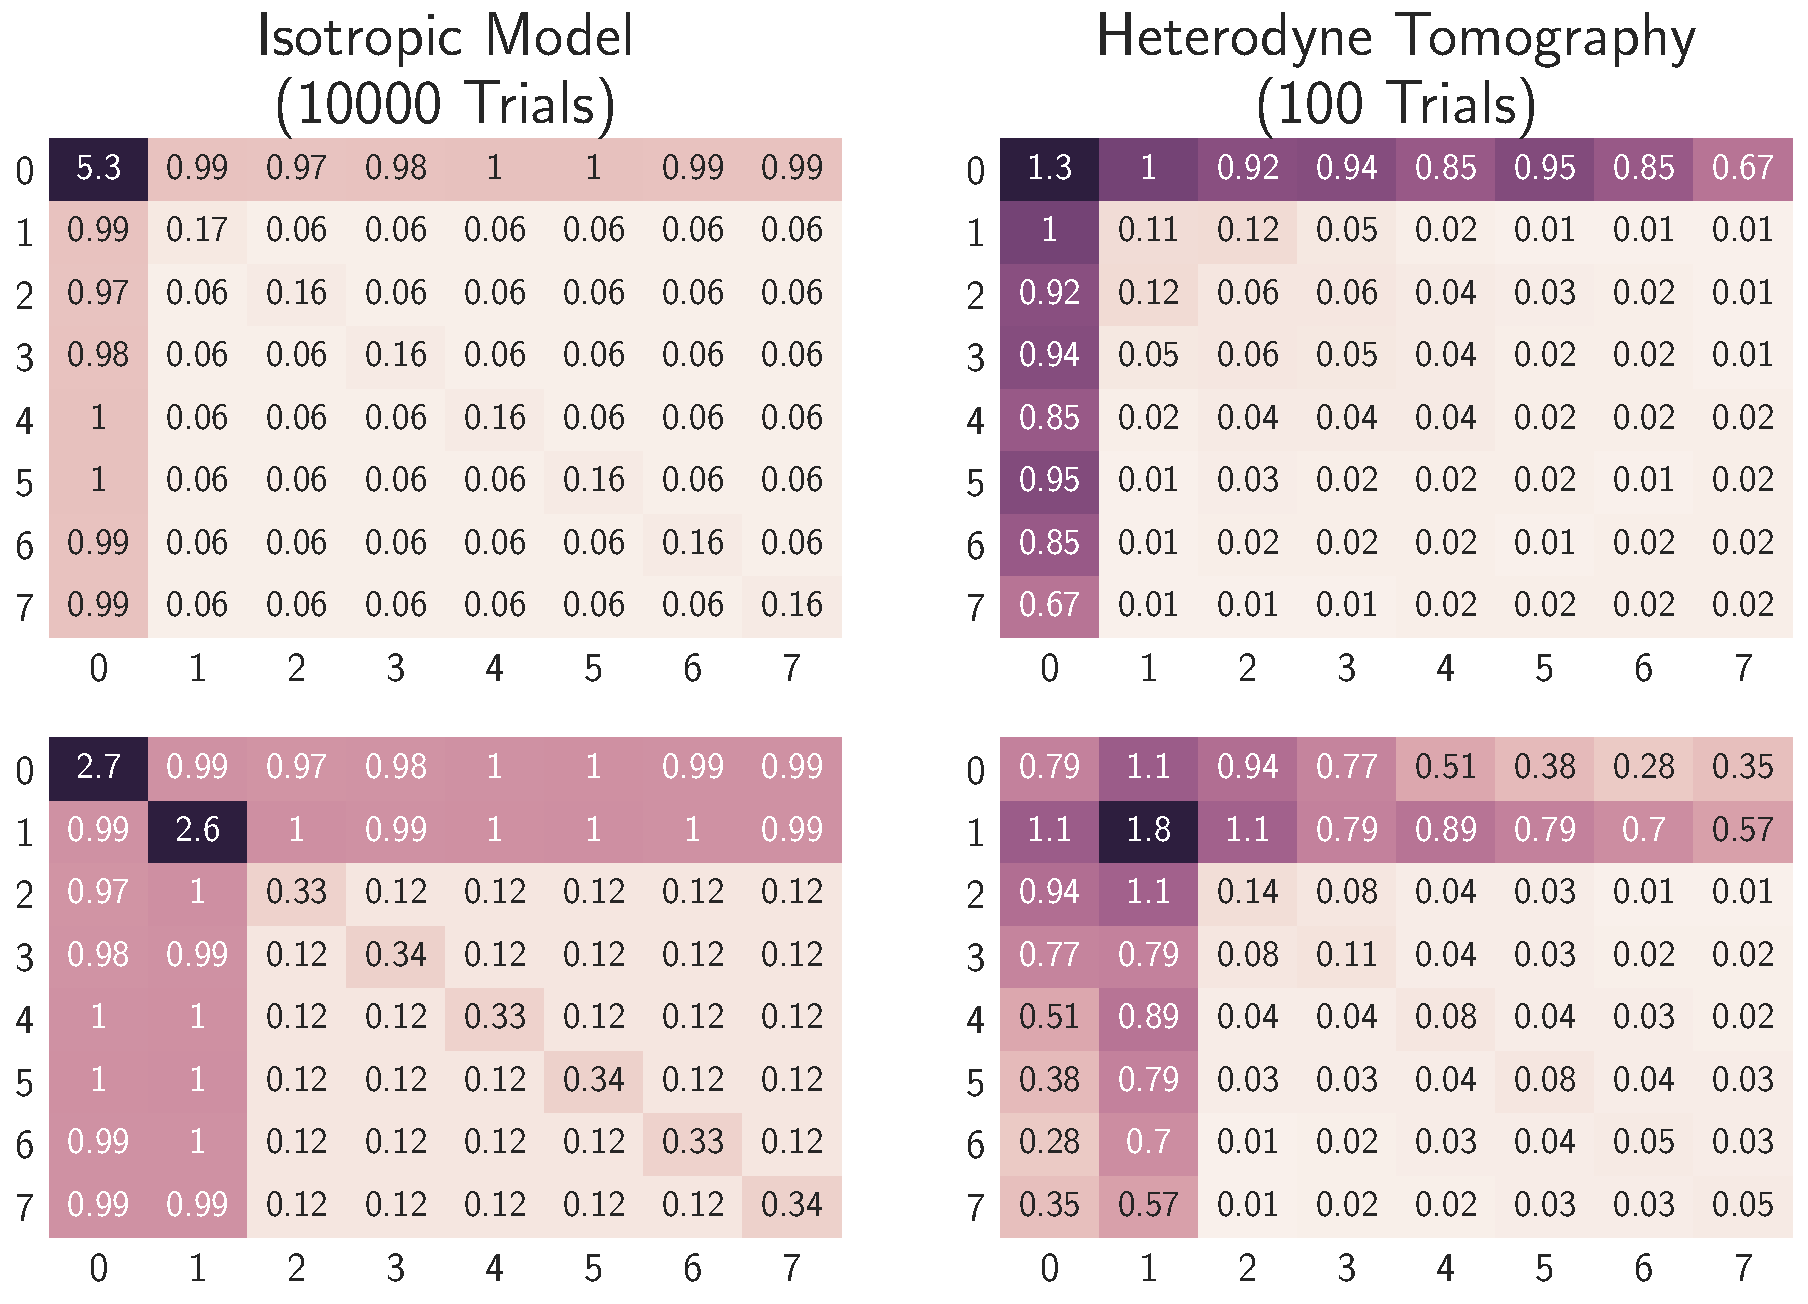
\includegraphics[width=\columnwidth]{Images/Figure_13.pdf}
 \caption{For Poisson-distributed data, the behavior of the loglikelihood ratio statistic depends strongly on the expected number of counts $\theta_{0}$. The single parameter in the Poisson model will be fully contributing -- i.e., $\langle \lambda \rangle = 1$ -- only when $\theta_{0} \gtrsim 5$. When $\theta_{0} << 1$, the parameter is ``under-contributing", as $\langle \lambda \rangle <<1$. As shown in the inset, there exists a regime $(1 \lesssim \theta_{0} \lesssim 5)$ 
where the parameter is ``super-contributing'' -- i.e., $1 \lesssim \langle \lambda \rangle \lesssim 1.2$.}
\label{fig:poissonbump}
\end{figure}

Curiously, we see that as $\theta_{0} \rightarrow 0^{+}$, $\langle \lambda \rangle \rightarrow 0$. Why is this the case? 
When the number of counts is 0, the parameter $\theta$ is not a ``parameter" at all, since it \emph{cannot fluctuate}. It has to be set to 0! Phrased another way, the Wilks Theorem establishes a conversion factor between fluctuating parameters and $\langle \lambda \rangle$. When parameters do not fluctuate very much, they do not contribute much to the statistic. Taken to the extreme, if a parameter cannot fluctuate at all, and the value it is pinned to happens to be the true value, then its scaled mean squared error is 0, so $\langle \lambda \rangle = 0$.

In heterodyne tomography, if we use a model with support in a $D$-dimensional Hilbert space $\M_{D}$, but the true state 
which generated the data has support on a $d < D$-dimensional Hilbert space, then the probability of observing any $
\alpha$ values with radius $r > \sqrt{d}$ drops off as $e^{-d}$. (Recall $\mathrm{Pr}(\alpha) = \frac{\langle \alpha | \rho | \alpha\rangle}{\pi}  \propto e^{-|\alpha|^{2}}$.) With very few ``counts'' out in this region in phase space, 
the additional $\mathcal{O}(D^{2}-d^{2})$ parameters we added do not fluctuate very much, and these parameters are 
``under-contributing" to the expected value of the loglikelihood ratio statistic. Conversely, in order for a parameter in $\M_{D}$ which has support on a high-energy Fock state $|n\rangle$, 
with $n > d$, to contribute to the loglikelihood ratio statistic, we may have to draw $e^{\mathcal{O}(n)}$ samples before its contribution is 1. 



\end{document}
